% Hak Cipta 2020 oleh Robert Hildebrand
%Karya ini dilisensikan berdasarkan
%Lisensi Internasional Creative Commons Atribusi-BerbagiSerupa 4.0 (CC BY-SA 4.0)
%Lihat http://creativecommons.org/licenses/by-sa/4.0/% 



%\documentclass[../open-optimization/open-optimization.tex]{subfiles}
% 
%\begin{document}

\chapter{Pengantar Formulasi Pemrograman Bilangan Bulat}
\label{sec:IP-formulations} 
\begin{outcome}
\begin{enumerate}
\item[A.] Mempelajari formulasi klasik pemrograman bilangan bulat.
\item[B.] Menunjukkan berbagai penggunaan variabel biner dan bilangan bulat.
\item[C.] Menunjukkan format pemodelan masalah optimisasi dengan himpunan, parameter, variabel, dan model.
\end{enumerate}
\end{outcome}

\begin{quote}
\itshape Program linier Anda menyarankan untuk membangun 2,7 gudang dan mengoperasikan 3,4 truk. Membulatkan ke atas menjadi 3 gudang dapat melampaui anggaran; membulatkan ke bawah menjadi 2 gudang dapat menyebabkan permintaan tidak terpenuhi; dan kedua rencana hasil pembulatan itu belum tentu mendekati rencana bilangan bulat terbaik. Lebih buruk lagi, banyak keputusan sama sekali bukan berupa kuantitas, melainkan pilihan (buka fasilitas ini atau tidak, tugaskan pekerjaan ini ke mesin itu atau tidak), sehingga ``0,7 dari jawaban ya'' tidak bermakna. Mengharuskan variabel bernilai bulat tampak seperti perubahan kecil terhadap program linier. Kenyataannya tidak demikian: perubahan itu memberikan daya pemodelan yang luar biasa, dan bab ini mengajak Anda melihat apa saja yang dapat dinyatakan oleh daya tersebut.
\end{quote}

%\begin{comment}
%Kita akan mempelajari teori kompleksitas pada bagian selanjutnya. Namun, perhatikan klasifikasi kompleksitas setiap masalah ( \polynomial,\npcomplete, \nphard) agar Anda memperoleh gambaran tentang tingkat kesulitannya. Istilah-istilah ini akan kita definisikan nanti.
%\end{comment}




Pada bagian ini, kita akan menguraikan formulasi klasik pemrograman bilangan bulat. Formulasi-formulasi ini dapat mencerminkan masalah dunia nyata secara persis atau menjadi bagian dari penyusunan suatu masalah dunia nyata.

\section{Masalah Ransel}
\emph{Masalah ransel} dapat memiliki bentuk berbeda, bergantung pada apakah variabelnya biner atau bilangan bulat. Versi biner berarti hanya ada satu barang dari setiap jenis barang yang dapat diambil. Masalah ini biasanya digambarkan sebagai sebuah ransel dan sejumlah barang yang akan dimasukkan ke dalamnya (lihat \autoref{fig:wiki-File-knapsack}), tetapi penerapannya mencakup banyak konteks.



 \includefigurestatic[Masalah Ransel: barang mana yang harus kita pilih untuk dimasukkan ke dalam ransel agar nilainya maksimum dengan tetap mematuhi batas berat 15 kg?][width=.4\linewidth][h]{wiki-File-knapsack}

\begin{general}{Masalah Ransel Biner}{\npcomplete}
Diberikan vektor bobot taknegatif $\a \in \Q^n_+$, kapasitas $b \in \Q_+$, dan koefisien objektif $\c \in \Q^n$,
\begin{equation}
\begin{split}
\max \ \ & \c^\top \x\\
\st \ \ & \a^\top \x \leq b\\
& \x \in \{0,1\}^n
\end{split}
\end{equation}
\end{general}
 


 
%\begin{figure}[H]
%\begin{center}
%\includegraphics[scale = 0.2]{knapsack}\footnotemark 
%\end{center}
%\label{fig:knapsack}
%\caption{Masalah Ransel: barang mana yang harus kita pilih untuk dimasukkan ke dalam ransel agar nilainya maksimum dengan tetap mematuhi batas berat 15 kg?}
%\end{figure}
%\footnotetext{\url{https://en.wikipedia.org/wiki/Knapsack_problem}}

\begin{examplewithallcode}{Ransel}
{}
{https://github.com/open-optimization/open-optimization-or-book/tree/master/Intro-Math-Programming/baseText/optimization/optimization-examples/knapsack_pulp.ipynb}
{https://github.com/open-optimization/open-optimization-or-book/tree/master/Intro-Math-Programming/baseText/optimization/optimization-examples/knapsack_gurobi.ipynb}
\label{example:knapsack}
Anda memiliki sebuah ransel (tas) yang hanya mampu menampung berat W = 15 kg. Ada 5 barang yang mungkin dimasukkan ke dalam ransel. Barang-barang tersebut (berat, nilai) adalah:
(12 kg, $\$$4), (2 kg, $\$$2), (1 kg, $\$$2), (1 kg, $\$$1), (4 kg, $\$$10). Barang mana yang harus Anda ambil untuk memaksimumkan nilai di dalam ransel? Lihat \autoref{fig:wiki-File-knapsack}.\\

\modelhead{Variabel}
\begin{itemize}
\item tetapkan $x_i = 1$ jika barang $i$ berada di dalam tas
\item tetapkan $x_i = 0$ jika barang $i$ tidak berada di dalam tas
\end{itemize}
\modelhead{Model}
\begin{align}
\max \quad & 4 x_1 + 2 x_2 + 2 x_3 + 1 x_4 + 10 x_5   \tag{Nilai total} \\
\st        & 12 x_1 + 2 x_2 + 1 x_3 + 1 x_4 + 4 x_5 \leq 15   \tag{Batas kapasitas} \\
& x_i \in \{0,1\} &&\quad \text{untuk semua } i=1, \dots, 5   \tag{Barang diambil atau tidak}
\end{align}
\end{examplewithallcode}
Untuk kasus bilangan bulat, biasanya kita mengharuskan variabel berupa bilangan bulat taknegatif, sehingga digunakan notasi $\x \in \Z^n_+$. Keadaan ini mencerminkan bahwa alih-alih memiliki barang satuan, terdapat jenis-jenis barang dan Anda dapat mengambil sebanyak apa pun dari setiap jenis selama memenuhi kendala.
\begin{general}{Masalah Ransel Bilangan Bulat}{\npcomplete}
Diberikan vektor bobot taknegatif $\a \in \Q^n_+$, kapasitas $b \in \Q_+$, dan koefisien objektif $c \in \Q^n$,
\begin{equation}
\begin{split}
\max \ \ & \c^\top \x\\
\st \ \ & \a^\top \x \leq b\\
& \x \in \Z^n_+
\end{split}
\end{equation}
\end{general}
Kita juga dapat mempertimbangkan versi dengan kendala kesamaan.
\begin{general}{Masalah Ransel Bilangan Bulat dengan Kendala Kesamaan}{\nphard}
Diberikan vektor bobot taknegatif $\a \in \Q^n_+$, kapasitas $b \in \Q_+$, dan koefisien objektif $c \in \Q^n$,
\begin{align}
\max \quad & \c^\top \x \\
\st        & \a^\top \x = b \\
& \x \in \Z^n_+
\end{align}
\end{general}



\begin{examplewithallcode}{Jumlah Koin Minimum}
{}
{https://github.com/open-optimization/open-optimization-or-book/tree/master/Intro-Math-Programming/baseText/optimization/optimization-examples/min_coins_pulp.ipynb}
{https://github.com/open-optimization/open-optimization-or-book/tree/master/Intro-Math-Programming/baseText/optimization/optimization-examples/min_coins_gurobi.ipynb}
\label{ex:min-coins}
Dengan menggunakan koin satu sen, lima sen, sepuluh sen, dan dua puluh lima sen, bagaimana Anda dapat meminimumkan jumlah koin yang diperlukan untuk membentuk nilai 83\textcent{}?

\modelhead{Variabel}
\begin{itemize}
\item Misalkan $p$ adalah jumlah koin satu sen yang digunakan
\item Misalkan $n$ adalah jumlah koin lima sen yang digunakan
\item Misalkan $d$ adalah jumlah koin sepuluh sen yang digunakan
\item Misalkan $q$ adalah jumlah koin dua puluh lima sen yang digunakan
\end{itemize}
\modelhead{Model}
\begin{align*}
\min \quad & p + n + d + q   \tag{jumlah total koin yang digunakan} \\
\st        & p + 5n + 10d + 25 q = 83 & \text{berjumlah } 83\,\text{\textcent} \\
& p,d,n,q \in \Z_+   \tag{masing-masing merupakan bilangan bulat taknegatif}
\end{align*}
\end{examplewithallcode}

\section{Penganggaran Modal}
\label{sec:capital-budgeting}

% Hak cipta Robert Hildebrand 2019

Masalah \emph{penganggaran modal} merupakan generalisasi yang berguna dari masalah ransel. Masalah ini memiliki struktur yang sama dengan masalah ransel, tetapi kini memiliki beberapa kendala. Mula-mula kita akan menjelaskan masalahnya, memberikan model umum, lalu meninjau sebuah contoh eksplisit.

\begin{general}{Penganggaran Modal}{}
\label{general:capital-budgeting}
Sebuah perusahaan memiliki $n$ proyek yang dapat dilaksanakan untuk memaksimumkan pendapatan, tetapi keterbatasan anggaran membuat tidak semua proyek dapat diselesaikan.
\begin{itemize}
\item Proyek $j$ diperkirakan menghasilkan pendapatan keseluruhan sebesar $c_j$ dolar.
\item Proyek $j$ memerlukan investasi sebesar $a_{ij}$ dolar pada periode waktu $i$, untuk $i = 1,\ldots,m$.
\item Modal yang tersedia untuk dibelanjakan pada periode waktu $i$ adalah $b_i$.
\end{itemize}
Proyek mana yang harus dibiayai perusahaan untuk memaksimumkan hasil yang diharapkan sambil memenuhi kendala anggaran mingguan?
\end{general}

\newpage

Mula-mula kita berikan rumusan umum masalah ini.

\begin{general}{Model Penganggaran Modal}{}
\noindent \textbf{Himpunan:}
\begin{itemize}
\item Misalkan $I = \{1, \dots, m\}$ adalah himpunan periode waktu.
\item Misalkan $J = \{1, \dots, n\}$ adalah himpunan investasi yang mungkin.
\end{itemize}

\noindent \textbf{Parameter:}
\begin{itemize}
\item $c_j$ adalah pendapatan yang diharapkan dari investasi $j$, untuk $j \in J$.
\item $b_i$ adalah modal yang tersedia pada periode waktu $i$, untuk $i$ di $I$.
\item $a_{ij}$ adalah sumber daya yang diperlukan untuk investasi $j$ pada periode waktu $i$, untuk $i$ di $I$ dan $j$ di $J$.
\end{itemize}

\noindent \textbf{Variabel:}
\begin{itemize}
\item tetapkan $x_j = 1$ jika investasi $j$ dipilih;
\item tetapkan $x_j = 0$ jika investasi $j$ tidak dipilih.
\end{itemize}
\textbf{Model:}
\begin{align*}
	\max ~~~& \sum_{j = 1}^n c_jx_j \tag{Total Pendapatan yang Diharapkan}\\
	s.t. ~~~&\sum_{j = 1}^n a_{ij}x_j\leq b_i, ~~~i = 1,\ldots,m \tag{Kendala sumber daya minggu $i$}\\
	& x_j \in \{0,1\} , \ j = 1,\ldots,n
	\end{align*}

\end{general}


\newpage
%\begin{examplewithcode}{Penganggaran Modal}{code:capital-budgeting}
%\label{example:capital-budgeting}
Perhatikan contoh pada tabel berikut.
	\begin{table}[h]
			\centering\small
			\begin{tabularx}{\textwidth}{|c|c|>{\raggedright\arraybackslash}X|>{\raggedright\arraybackslash}X|}%[<+->]
				\hline
				Proyek & $\mathbb{E}$[Pendapatan] & Sumber daya yang diperlukan pada minggu 1 & Sumber daya yang diperlukan pada minggu 2\\\hline
				\rowcolor{gray!10} 1 & 10 & 3 & 4\\
				\hline
				2 & 8 & 1 & 2\\\hline
				\rowcolor{gray!10} 3 & 6 & 2 & 1\\
				\hline
				Sumber daya tersedia & & 5 & 6\\
				\hline
		\end{tabularx}
	\end{table}


Berdasarkan data ini, kita dapat menyusun masalah secara eksplisit sebagai berikut.

\begin{examplewithallcode}{Penganggaran Modal}{}{https://github.com/open-optimization/open-optimization-or-examples/blob/master/integer-programming/capital-budgeting.ipynb}{}
\noindent \textbf{Himpunan:}
\begin{itemize}
\item Misalkan $I = \{1,2\}$ adalah himpunan periode waktu.
\item Misalkan $J = \{1, 2,3\}$ adalah himpunan investasi yang mungkin.
\end{itemize}

\noindent \textbf{Parameter:}
\begin{itemize}
\item $c_j$ diberikan pada kolom ``$\mathbb{E}$[Pendapatan]''.
\item $b_i$ diberikan pada baris ``Sumber daya tersedia''.
\item $a_{ij}$ diberikan pada baris $j$ dan kolom untuk minggu $i$.
\end{itemize}

\noindent \textbf{Variabel:}
\begin{itemize}
\item tetapkan $x_j = 1$ jika investasi $j$ dipilih;
\item tetapkan $x_j = 0$ jika investasi $j$ tidak dipilih.
\end{itemize}

Model eksplisitnya adalah\\
\noindent \textbf{Model:}
\begin{align*}
	\max\ \ \  & 10x_1+8x_2+6x_3 \tag{Total Pendapatan yang Diharapkan}\\
	s.t. \ \ &
	3x_1+1x_2+2x_3\leq5 \tag{Kendala sumber daya minggu 1}\\
	&4x_1+2x_2+1x_3\leq6 \tag{Kendala sumber daya minggu 2}\\
&x_j \in \{0,1\},\  j = 1,2,3
\end{align*}

\end{examplewithallcode}


\section{Masalah Penentuan Ukuran Lot Berkapasitas (CLSP)}

\textit{Masalah Penentuan Ukuran Lot Berkapasitas (Capacitated Lot Sizing Problem, CLSP)} adalah masalah optimisasi mendasar dalam perencanaan produksi. Tujuannya ialah menentukan jadwal produksi optimal yang meminimumkan biaya total sekaligus mematuhi kendala kapasitas. Fungsi objektif memperhitungkan biaya produksi, biaya penyiapan, dan biaya penyimpanan persediaan selama suatu horizon perencanaan.

Misalkan \( T \) menyatakan jumlah periode waktu diskret, yang diindeks oleh \( t \in \{1,2,\dots,T\} \). Parameter masalah didefinisikan sebagai berikut:
\begin{itemize}
    \item \( d_t \) adalah permintaan pada periode \( t \),
    \item \( p_t \) menyatakan biaya produksi per unit,
    \item \( f_t \) adalah biaya tetap penyiapan yang dikeluarkan jika produksi berlangsung,
    \item \( h_t \) menyatakan biaya penyimpanan persediaan per unit, dan
    \item \( c_t \) menyatakan kapasitas produksi maksimum pada periode \( t \).
\end{itemize}

Variabel keputusannya adalah:
\begin{itemize}
    \item \( x_t \) menyatakan kuantitas yang diproduksi pada periode \( t \),
    \item \( s_t \) adalah tingkat persediaan pada akhir periode \( t \), dan
    \item \( y_t \) adalah variabel biner yang bernilai 1 jika produksi berlangsung pada periode \( t \), dan 0 jika tidak.
\end{itemize}

CLSP dapat dirumuskan sebagai program linier bilangan bulat campuran berikut:
\begin{align}
\min \quad & \sum_{t=1}^{T} \left( p_t x_t + f_t y_t + h_t s_t \right)   \tag{Minimumkan biaya total}\label{eq:clsp-objective} \\
\st        & s_{t-1} + x_t - d_t = s_t &&\quad \text{untuk semua } t = 1,2,\dots,T   \tag{Keseimbangan persediaan}\label{eq:clsp-inventory} \\
    & x_t \leq y_t c_t &&\quad \text{untuk semua } t = 1,2,\dots,T   \tag{Kendala kapasitas dan penyiapan}\label{eq:clsp-capacity} \\
    & x_t, s_t \geq 0 &&\quad \text{untuk semua } t = 1,2,\dots,T   \tag{Kendala ketaknegatifan}\label{eq:clsp-nonnegativity} \\
    & y_t \in \{0,1\} &&\quad \text{untuk semua } t = 1,2,\dots,T   \tag{Keputusan produksi biner}\label{eq:clsp-binary}
\end{align}

Fungsi objektif \eqref{eq:clsp-objective} meminimumkan biaya total sepanjang horizon perencanaan dengan mencakup biaya produksi, penyiapan, dan penyimpanan persediaan. Kendala keseimbangan persediaan \eqref{eq:clsp-inventory} memastikan bahwa permintaan pada setiap periode dipenuhi menggunakan persediaan dari periode sebelumnya atau unit yang baru diproduksi. Kendala \eqref{eq:clsp-capacity} menerapkan batas kapasitas produksi dan memastikan bahwa biaya penyiapan dikeluarkan ketika produksi berlangsung. Kendala \eqref{eq:clsp-nonnegativity} menerapkan ketaknegatifan pada tingkat produksi dan persediaan, sedangkan \eqref{eq:clsp-binary} memastikan bahwa keputusan penyiapan bersifat biner.

Demi kesederhanaan, kita mengasumsikan tingkat persediaan awal sebesar nol.

\section{Penentuan Lokasi Fasilitas}
\label{sec:facility-location}
Model dasar masalah penentuan lokasi fasilitas menentukan tempat untuk menempatkan toko atau fasilitas agar dekat dengan semua pelanggan sehingga biaya transportasi ke pelanggan berkurang. Setiap pelanggan diketahui memiliki sejumlah permintaan untuk suatu produk, dan setiap fasilitas memiliki kapasitas yang membatasi banyaknya permintaan tersebut yang dapat dipenuhi. Kita juga perlu mempertimbangkan biaya pembangunan fasilitas di lokasi tertentu.

Kerangka dasar ini dapat diterapkan pada banyak jenis masalah dan memiliki sejumlah variasi. Di sini kita menyajikan \emph{masalah penentuan lokasi fasilitas berkapasitas}. Variasi tambahan dan formulasi alternatif dibahas dalam Buku 2.



\subsection{Penentuan Lokasi Fasilitas Berkapasitas}

\begin{general}{Penentuan Lokasi Fasilitas Berkapasitas 1}{\npcomplete}
Diberikan biaya hubungan \( c_{ij} \), biaya tetap pembangunan \( f_i \), permintaan \( d_j \), dan kapasitas fasilitas \( u_i \), masalah \textbf{penentuan lokasi fasilitas berkapasitas} dirumuskan sebagai berikut:

\modelhead{Himpunan}
\begin{itemize}
\item Misalkan \( I = \{1,\dots, n\} \) adalah himpunan fasilitas.
\item Misalkan \( J = \{1, \dots, m\} \) adalah himpunan pelanggan.
\end{itemize}

\modelhead{Parameter}
\begin{itemize}
\item \( f_i \) — biaya membuka fasilitas \( i \).
\item \( c_{ij} \) — biaya melayani satu unit permintaan pelanggan \( j \) dari fasilitas \( i \).
\item \( u_i \) — kapasitas (dalam unit) fasilitas \( i \).
\item \( d_j \) — total permintaan (dalam unit) pelanggan \( j \).
\end{itemize}

\modelhead{Variabel}
\begin{itemize}
\item \( y_i \in \{0,1\} \) — sama dengan 1 jika fasilitas \( i \) dibuka; 0 jika tidak.
\item \( x_{ij} \geq 0 \) — jumlah unit permintaan pelanggan \( j \) yang dilayani oleh fasilitas \( i \).
\end{itemize}

\modelhead{Model}
\begin{align}
\min \quad & \sum_{i=1}^n \sum_{j=1}^m c_{ij} x_{ij} + \sum_{i=1}^n f_i y_i   \tag{Biaya total} \\
\st        & \sum_{i=1}^n x_{ij} = d_j &&\quad \text{untuk semua } j = 1,\dots,m   \tag{Penuhi permintaan} \\
& \sum_{j=1}^m x_{ij} \leq u_i y_i &&\quad \text{untuk semua } i = 1,\dots,n   \tag{Kapasitas fasilitas} \\
& x_{ij} \geq 0 &&\quad \text{untuk semua } i = 1,\dots,n,\; j = 1,\dots,m   \tag{Ketaknegatifan} \\
& y_i \in \{0,1\} &&\quad \text{untuk semua } i = 1,\dots,n   \tag{Buka fasilitas}
\end{align}

\end{general}

% ============================================================================
% Formulasi tambahan untuk penentuan lokasi fasilitas dibahas dalam Buku 2
% ============================================================================
% CATATAN: teks Masalah Penugasan Terampat di dalam blok \iffalse berikut
% diadaptasi dari Wikipedia (CC BY-SA). Sebelum mengaktifkannya kembali, tambahkan
% atribusi yang semestinya (nama artikel, lisensi, perubahan yang dibuat) atau tulis ulang dari awal.
\iffalse  % BEGIN BOOK 2 ONLY - Alternative Formulations
Selanjutnya, kita menyajikan metode yang memodelkannya dengan melacak fraksi permintaan yang dilayani.
\begin{general}{Penentuan Lokasi Fasilitas Berkapasitas 2}{\npcomplete}
Diberikan biaya hubungan $c_{ij}$ dan biaya tetap pembangunan $f_i$, permintaan $d_j$, serta kapasitas $u_i$, masalah penentuan lokasi fasilitas berkapasitas adalah

\modelhead{Himpunan}
\begin{itemize}
\item Misalkan $I = \{1,\dots, n\}$ adalah himpunan fasilitas.
\item Misalkan $J = \{1, \dots, m\}$ adalah himpunan pelanggan.
\end{itemize}

\modelhead{Parameter}
\begin{itemize}
\item $f_i$ - biaya membuka fasilitas $i$.
\item $c_{ij}$ - biaya memenuhi seluruh permintaan pelanggan $j$ dari fasilitas $i$.
\item $u_{i}$ - kapasitas fasilitas $i$.
\item $d_{j}$ - permintaan pelanggan $j$.
%\item $c_j$ diberikan dalam kolom "$\mathbb{E}$[Pendapatan]".
%\item $b_i$ diberikan dalam baris "Sumber daya yang tersedia".
%\item $a_{ij}$ diberikan dalam baris $j$, dan kolom untuk minggu $i$.
\end{itemize}

\modelhead{Variabel}
\begin{itemize}
\item Misalkan
\begin{equation*}
y_{i} = \begin{cases}
1 & \text{jika kita membuka fasilitas $i$,}\\
0 & \text{jika tidak.}
\end{cases}
\end{equation*}
\item Misalkan $x_{ij} \geq 0$ adalah fraksi permintaan pelanggan $j$ yang dipenuhi oleh fasilitas $i$.
%\item tetapkan $x_i = 1$ jika investasi $i$ tidak dipilih
\end{itemize}

\modelhead{Model}
\begin{align}
\min \quad & \displaystyle\sum_{i=1}^n\sum_{j=1}^mc_{ij}x_{ij}+\sum_{i=1}^nf_iy_i   \tag{biaya total} \\
\st        & \displaystyle\sum_{i=1}^nx_{ij}=1 &&\quad \text{untuk semua } j=1,\dots,m   \tag{tetapkan permintaan ke fasilitas} \\
& \displaystyle \sum_{j=1}^md_jx_{ij}\leq u_iy_i &&\quad \text{untuk semua } i=1\dots,n   \tag{kapasitas fasilitas $i$} \\
& x_{ij}\geqslant0 &&\quad \text{untuk semua } i=1,\dots,n \text{ dan }j=1,\dots,m   \tag{fraksi taknegatif dari permintaan yang dipenuhi} \\
& y_i\in\{0,1\} &&\quad \text{untuk semua } i=1,\dots,n   \tag{fasilitas dibuka/tidak dibuka}
\end{align}

\end{general}

Terakhir, kita menyajikan versi yang memiliki variabel sama, tetapi kendalanya memodelkan solusi layak dengan cara yang sedikit berbeda.

\begin{align*}
\min \quad & \sum_{i = 1}^m\sum_{j=1}^n c_{ij}x_{ij}+\sum_{i = 1}^mf_iy_i \\
\st        & \sum_{i = 1}^mx_{ij} = 1,~~~~~j =1,\ldots n \\
& \displaystyle \sum_{j=1}^md_jx_{ij}\leq u_i &&\quad \text{untuk semua } i=1\dots,n   \tag{kapasitas fasilitas $i$} \\
& x_{ij}\leq y_i,~~~~~ i = 1,\ldots m,~~~ j = 1,\ldots,n \\
& x_{ij} \geq 0~~~~~ i = 1,\ldots,m, ~~~j = 1,\ldots,n \\
& y_i\in \{0,1\}, \  \  i = 1,\ldots,m
\end{align*}
\fi  % END BOOK 2 ONLY - Alternative Formulations

\begin{examplewithcode}{Penentuan Lokasi Fasilitas Berkapasitas: Contoh Distribusi Ritel}{\href{https://github.com/open-optimization/open-optimization-or-examples/blob/master/integer-programming/facility-location-capacitated.ipynb}{Gurobipy}}

\textbf{Konteks:} Sebuah perusahaan ritel berencana mendirikan pusat-pusat distribusi di seluruh negeri untuk melayani tokonya secara efisien. Perusahaan harus memutuskan pusat distribusi mana yang akan dibuka dan toko mana yang harus dilayani oleh setiap pusat. Biaya pembukaan setiap pusat dan pelayanan toko dari pusat tersebut telah diketahui, dan setiap pusat memiliki kapasitas maksimum. Permintaan setiap toko juga telah diketahui.

\textbf{Data yang Diberikan:} (\href{https://github.com/open-optimization/open-optimization-or-examples/blob/master/integer-programming/distribution-data.xlsx}{distribution-data.xlsx})

\begin{itemize}
    \item Jumlah calon pusat distribusi ($n$): 3
    \item Jumlah toko ($m$): 4
\end{itemize}


\begin{table}[ht]
\centering
\caption{Data Gabungan Pusat Distribusi dan Toko}
\begin{tabular}{lcc|cccc}
\toprule
 & \(\mathbf{f_i}\) & \(\mathbf{u_i}\) & \multicolumn{4}{c}{\(\mathbf{c_{ij}}\) (Biaya Melayani Toko)} \\
\cmidrule(lr){4-7}
\textbf{Pusat} & (\$) & (unit) & Toko 1 & Toko 2 & Toko 3 & Toko 4 \\
\midrule
Pusat 1 & 150,000 & 100 & \$50 & \$60 & \$70 & \$85 \\
Pusat 2 & 100,000 & 80  & \$75 & \$45 & \$55 & \$50 \\
Pusat 3 & 180,000 & 90  & \$65 & \$80 & \$40 & \$60 \\
\midrule
\textbf{Permintaan Toko \(d_j\)} & & & 400 & 300 & 200 & 250 \\
\bottomrule
\end{tabular}
\end{table}

\textbf{Formulasi Model:}
Model penentuan lokasi fasilitas berkapasitas yang dijelaskan sebelumnya dapat diterapkan pada skenario ini dengan data yang diberikan untuk menentukan jumlah dan lokasi optimal pusat distribusi yang akan dibuka, serta toko-toko yang harus dilayani oleh setiap pusat.
\begin{center}
\includegraphicbook[scale = 0.75]{facility-location}\par\captionof{figure}{Diagram jaringan untuk penentuan lokasi fasilitas: tiga calon pusat distribusi yang terhubung ke toko-toko.}\label{fig:facility-location}% fig-num-auto

\end{center}
\end{examplewithcode}

Jika Anda menyusun dan menyelesaikan contoh ini, Anda akan menemukan bahwa contoh tersebut tidak layak: total permintaan toko adalah $1150$ unit, sedangkan ketiga pusat secara bersama-sama hanya dapat memasok paling banyak $270$. Hal ini disengaja. Tidak setiap masalah memiliki solusi yang baik, dan ditemukannya ketidaklayakan itu sendiri merupakan informasi berguna yang diberikan oleh sebuah model. Sebagai latihan, tentukan cara memperbaiki contoh tersebut: kurangi permintaan atau tambahkan kapasitas.

% ============================================================================
% Penentuan Lokasi Fasilitas Tanpa Kapasitas dibahas dalam Buku 2
% ============================================================================
\iffalse  % BEGIN BOOK 2 ONLY - Uncapacitated Facility Location
\subsection{Penentuan Lokasi Fasilitas Tanpa Kapasitas}
\begin{general}{Penentuan Lokasi Fasilitas Tanpa Kapasitas}{\npcomplete}
Diberikan biaya hubungan $c_{ij}$ dan biaya tetap pembangunan $f_i$, masalah penentuan lokasi fasilitas tanpa kapasitas adalah
\begin{equation}
\begin{array}{rl}
\min & \displaystyle\sum_{i=1}^n\sum_{j=1}^mc_{ij}z_{ij}+\sum_{i=1}^nf_ix_i \\
\st & \displaystyle\sum_{i=1}^nz_{ij}=1 \text{ untuk semua }j=1,\dots,m \\
& \displaystyle \sum_{j=1}^mz_{ij}\leq Mx_i\text{ untuk semua }i=1\dots,n \\
&z_{ij}\in\{0,1\}\text{ untuk semua }i=1,\dots,n \text{ dan }j=1,\dots,m\\
&x_i\in\{0,1\}\text{ untuk semua } i=1,\dots,n
\end{array}
\end{equation}
Di sini $M$ adalah bilangan besar dan dapat dipilih sebagai $M = m$, tetapi nilainya dapat diperkecil jika lebih banyak konteks diketahui.
\end{general}

Model alternatif!

\begin{equation}
\begin{array}{rl}
\min & \displaystyle\sum_{i=1}^n\sum_{j=1}^mc_{ij}z_{ij}+\sum_{i=1}^nf_ix_i \\
\st & \displaystyle\sum_{i=1}^nz_{ij}=1 \text{ untuk semua }j=1,\dots,m \\
& z_{ij}\leq x_i\text{ untuk semua }i=1\dots,n \text{ untuk semua } j = 1, \dots, m \\
&z_{ij}\in\{0,1\}\text{ untuk semua }i=1,\dots,n \text{ dan }j=1,\dots,m\\
&x_i\in\{0,1\}\text{ untuk semua } i=1,\dots,n
\end{array}
\end{equation}
\newpage
\fi  % END BOOK 2 ONLY - Uncapacitated Facility Location


\begin{casestudybox}{Di Mana Pesawat Pengebom Air Harus Bermalam? Penentuan Pangkalan Pesawat Tanker di Ontario}
\label{case:wildfire-airtankers}

Ontario memadamkan kebakaran hutan dengan armada pesawat tanker (pengebom air). Kebakaran yang tertangani dalam beberapa jam pertama biasanya hanya menjadi kejadian kecil; kebakaran yang terlewat akan berkembang menjadi bencana besar. Karena itu, kemampuan provinsi untuk menangani kebakaran baru dengan cepat bergantung pada lokasi pangkalan pesawat tanker setiap pagi. Pada awal 1990-an, Kementerian Sumber Daya Alam Ontario meminta peneliti operasi membantu menentukan pangkalan utama. Model pemrograman matematis yang dihasilkan kemudian menjadi dasar strategi pangkalan provinsi tersebut sejak musim kebakaran 1993.

\subsection*{Tantangan}
Kebakaran tidak memberi tahu di mana ia akan bermula. Yang diketahui adalah pola historisnya: beberapa zona pengelolaan kebakaran mengalami jauh lebih banyak kebakaran awal daripada zona lain, dan pesawat tanker hanya dapat melakukan \emph{serangan awal} yang efektif terhadap kebakaran dalam jarak terbang terbatas dari pangkalannya. Dengan armada yang tetap, di mana pesawat harus ditempatkan agar sebanyak mungkin aktivitas kebakaran yang diperkirakan berada dalam jangkauan?

\subsection*{Solusi: Model Lokasi Cakupan}
\textbf{Jenis model: program bilangan bulat (lokasi fasilitas/cakupan). Tanpa pembelajaran mesin; masukan frekuensi kebakaran berupa rata-rata historis.}

\modelhead{Himpunan dan Parameter}
\begin{itemize}
\item Misalkan $I$ adalah himpunan zona pengelolaan kebakaran dan $J$ adalah himpunan calon pangkalan.
\item Misalkan $n_i$ adalah jumlah kebakaran yang diperkirakan di zona $i$ (berdasarkan catatan historis).
\item Misalkan $t_{ij} = 1$ jika pesawat tanker yang berpangkalan di $j$ dapat mencapai zona $i$ dalam standar waktu serangan awal, dan $0$ jika tidak.
\item Misalkan $N$ adalah jumlah pesawat tanker dalam armada.
\end{itemize}

\modelhead{Variabel}
\begin{itemize}
\item Misalkan $y_j \in \mathbb{Z}_{\geq 0}$ adalah jumlah pesawat tanker yang berpangkalan di $j$.
\item Misalkan $z_i = 1$ jika zona $i$ dicakup oleh setidaknya satu pangkalan dalam jangkauan.
\end{itemize}

\modelhead{Model}
\begin{align*}
\max \quad & \sum_{i \in I} n_i \, z_i   \tag{perkiraan kebakaran dalam jangkauan} \\
\st        & z_i \leq \sum_{j \in J} t_{ij}\, y_j &&\quad \text{untuk semua } i \in I   \tag{cakupan memerlukan pangkalan terdekat} \\
             & \sum_{j \in J} y_j = N   \tag{ukuran armada} \\
             & y_j \in \mathbb{Z}_{\geq 0}, \quad z_i \in \{0,1\}.
\end{align*}

\subsection*{Asumsi dan Penyederhanaan}
\begin{itemize}
\item Versi di atas menghitung sebuah zona sebagai tercakup atau tidak; model yang diterbitkan lebih terperinci, dengan memperhitungkan \emph{berapa banyak} pesawat yang dapat merespons dan variasi cuaca kebakaran harian.
\item Perkiraan jumlah kebakaran menggantikan kejadian kebakaran yang sebenarnya (acak): model mengoptimalkan hari rata-rata, bukan hari terburuk.
\item Pesawat tanker dapat dipindahkan antarpangkalan dari hari ke hari; karya yang diterbitkan memperlakukan pangkalan utama (musiman) dan penempatan harian sebagai keputusan yang saling terkait.
\end{itemize}

\subsection*{Implementasi dan Hasil}
Kementerian Sumber Daya Alam Ontario menggunakan model tersebut sebagai dasar strategi pangkalan utama pesawat tankernya mulai musim kebakaran 1993. Sejak itu, program pengelolaan kebakaran Ontario terus bekerja sama dengan peneliti operasi selama puluhan tahun dalam perencanaan penempatan, pengiriman, dan patroli deteksi.

\subsection*{Referensi}
\begin{itemize}
\item J.I. MacLellan, D.L. Martell. ``Basing Airtankers for Forest Fire Control in Ontario.'' \emph{Operations Research} 44(5), 677--686, 1996. \url{https://doi.org/10.1287/opre.44.5.677}
\item D.L. Martell. ``The Development and Implementation of Forest Fire Management Decision Support Systems in Ontario, Canada.'' \emph{Forest Ecology and Management} / catatan retrospektif, 2015.
\item D.L. Martell, R.J. Drysdale, G.E. Doan, D. Boychuk. ``An Evaluation of Forest Fire Initial Attack Resources.'' \emph{Interfaces} 14(5), 20--32, 1984.
\end{itemize}
\end{casestudybox}

\section{Penutupan Himpunan}

Masalah \emph{penutupan himpunan} dapat digunakan untuk beragam masalah. Kita akan melihat beberapa contoh pada bagian ini.

\begin{general}{Penutupan Himpunan}{\npcomplete}
\label{general:set-covering}
Diberikan himpunan $V$ dengan subhimpunan $V_1, \dots, V_l$, tentukan subhimpunan terkecil $S \subseteq V$ sedemikian sehingga
$S \cap V_i \neq \emptyset$ untuk semua $i=1, \dots, l$.

Masalah penutupan himpunan dapat dimodelkan sebagai
\begin{equation}
\begin{split}
\min \ \ & \one^\top x\\
\st \ \ & \sum_{v \in V_i} x_v \geq 1 \text{ untuk semua } i =1, \dots, l \\ 
& x_v \in \{0,1\} \text{ untuk semua } v \in V
\end{split}
\end{equation}
dengan $x_v$ sebagai variabel 0/1 yang bernilai $1$ jika kita memasukkan unsur $v$ ke dalam himpunan $S$, dan $0$ jika tidak memasukkannya ke dalam himpunan $S$.
\end{general}

%
%\begin{examplewithcode}{Penganggaran Modal}{https://github.com/open-optimization/open-optimization-or-examples/blob/master/integer-programming/capital-budgeting.ipynb}
%\noindent \textbf{Himpunan:}
%\begin{itemize}
%\item Misalkan $I = \{1,2\}$ adalah himpunan periode waktu.
%\item Misalkan $J = \{1, 2,3\}$ adalah himpunan investasi yang mungkin.
%\end{itemize}
%
%\noindent \textbf{Parameter:}
%\begin{itemize}
%\item $c_j$ diberikan dalam kolom "$\mathbb{E}$[Pendapatan]".
%\item $b_i$ diberikan dalam baris "Sumber daya yang tersedia".
%\item $a_{ij}$ diberikan dalam baris $j$, dan kolom untuk minggu $i$.
%\end{itemize}
%
%\noindent \textbf{Variabel:}
%\begin{itemize}
%\item tetapkan $x_i = 0$ jika investasi $i$ dipilih
%\item tetapkan $x_i = 1$ jika investasi $i$ tidak dipilih
%\end{itemize}
%
%Model eksplisit diberikan oleh\\
%\noindent  \textbf{Model:}
%\begin{align*}
%	\max\ \ \  & 10x_1+8x_2+6x_3 \tag{Total Pendapatan yang Diharapkan}\\
%	s.t. \ \ & 
%	3x_1+1x_2+2x_3\leq5 \tag{ Kendala sumber daya minggu 1}\\
%	&4x_1+2x_2+1x_3\leq6 \tag{ Kendala sumber daya minggu 2}\\
%&x_j \in \{0,1\},\  j = 1,2,3
%\end{align*}
%
%\end{examplewithcode}
%



Salah satu jenis khusus masalah penutupan himpunan adalah masalah \emph{penutup simpul}.
\begin{general}{Contoh: Penutup Simpul}{\npcomplete}
\label{ex:vertex-cover}
Diberikan graf $G = (V,E)$ yang terdiri atas simpul dan sisi, kita ingin mencari subhimpunan berukuran paling kecil $S \subseteq V$ sedemikian sehingga untuk setiap $e = (v,u) \in E$, $u$ atau $v$ berada dalam $S$.

Kita dapat menuliskannya sebagai program matematis dalam bentuk:
\begin{equation}
\begin{split}
\min \ \ & \one^\top x\\
\st \ \ & x_u + x_v \geq 1 \text{ untuk semua } (u,v) \in E \\ 
& x_v \in \{0,1\} \text{ untuk semua } v \in V.
\end{split}
\end{equation}
\end{general}




\begin{examplewithcode}{Penutupan himpunan: penempatan stasiun pemadam kebakaran}{https://github.com/open-optimization/open-optimization-or-examples/blob/master/integer-programming/fire-station-covering.ipynb}
\label{example:fire-station}

Dalam masalah stasiun pemadam kebakaran, kita berupaya memilih lokasi stasiun sedemikian sehingga setiap distrik memiliki stasiun pemadam kebakaran atau bertetangga dengan distrik yang memilikinya. Gambar~\ref{fig:tikz-Illustration1.pdf} menggambarkan himpunan distrik dan contoh penempatan lokasi stasiun pemadam kebakaran. Bagaimana kita dapat meminimumkan jumlah total stasiun pemadam kebakaran yang diperlukan?


\modelhead{Himpunan}
\begin{itemize}
\item Misalkan $V$ adalah himpunan distrik ($V = \{1, \dots, 16\}$)
\item Misalkan $V_i$ adalah himpunan distrik yang bertetangga dengan distrik $i$ (misalnya $V_1 = \{2,4,5\}$).
\end{itemize}

\modelhead{Variabel}
\begin{itemize}
\item tetapkan $x_i = 1$ jika distrik $i$ dipilih untuk memiliki stasiun pemadam kebakaran.
\item tetapkan $x_i = 0$ jika tidak.
\end{itemize}
\modelhead{Model}
\begin{align}
\min \quad & \sum_{i \in V} x_i \tag{ \# \text{ stasiun pemadam yang dibuka}} \\
\st        & x_i + \sum_{j \in V_i} x_j \geq 1 &&\quad \text{untuk semua } {i \in V}   \tag{Persyaratan kedekatan stasiun} \\
& x_i \in \{0,1\} &&\quad \text{untuk semua } i\in V   \tag{stasiun dibuka atau ditutup}
\end{align}
\end{examplewithcode}

\includefigurebooksource[Tata letak distrik dan kemungkinan lokasi stasiun pemadam kebakaran.][][h]{tikz-Illustration1.pdf}
\includefigurebooksource[Representasi penutupan himpunan untuk masalah stasiun pemadam kebakaran. Sebagai contoh, memilih distrik 16 untuk memiliki stasiun pemadam kebakaran mencakup distrik 13, 15, dan 16.]{tikz-Illustration2.pdf}
\includefigurebooksource[Representasi graf untuk masalah stasiun pemadam kebakaran. Setiap simpul terhubung oleh sebuah sisi ke simpul yang dipilih.]{tikz-Illustration3.pdf}

Gambar~\ref{fig:tikz-Illustration2.pdf} menunjukkan bagaimana struktur ketetanggaan diterjemahkan menjadi sebuah contoh penutupan himpunan, sedangkan Gambar~\ref{fig:tikz-Illustration3.pdf} memberikan tampilan graf yang ekuivalen untuk solusi yang sama.



%\documentclass[../open-optimization/open-optimization.tex]{subfiles}

%%%%%%%%%
%\begin{document}
%%%%%%%%%

\begin{general}{Penutupan Himpunan -- Deskripsi Matriks}{\npcomplete}
\label{general:set-covering-alternate}
Diberikan matriks nonnegatif $A \in \{0,1\}^{m \times n}$, sebuah vektor nonnegatif, dan vektor objektif $c \in \R^n$, masalah penutupan himpunan adalah
\begin{equation}
\begin{split}
\min \ \ & c^\top x\\
\text{s.t.} \ \ & Ax \geq \one \\
& x \in \{0,1\}^n.
\end{split}
\end{equation}
\end{general}
\begin{examplewithoutcode}{Penutupan Simpul dengan Matriks}{code:vertex-cover-matrix}
Cara lain untuk menyelesaikan \nameref{ex:vertex-cover} adalah dengan mendefinisikan \emph{matriks insidensi} $A$ dari graf tersebut. Matriks insidensi adalah matriks berukuran $|E| \times |V|$ dengan entri $\{0,1\}$. Setiap baris bersesuaian dengan sebuah sisi $e$, dan setiap kolom bersesuaian dengan sebuah simpul $v$. Untuk sisi $e = (u,v)$, baris yang bersesuaian memiliki nilai $1$ pada kolom-kolom yang bersesuaian dengan simpul $u$ dan $v$, serta nilai 0 di semua tempat lainnya. Dengan demikian, setiap baris memiliki tepat dua nilai 1. Penerapan rumusan di atas dalam \nameref{general:set-covering-alternate} memodelkan masalah tersebut.
\end{examplewithoutcode}




%%%%%%%%%
%\end{document}
%%%%%%%%%





\subsection{Penutupan (Perampatan Penutupan Himpunan)}
Kita juga dapat memperbolehkan jenis penutupan himpunan yang lebih umum, yaitu dengan variabel bilangan bulat taknegatif dan ruas kanan yang nilainya tidak hanya $1$.
\begin{general}{Penutupan}{\npcomplete}
\label{general:covering}
Diberikan matriks taknegatif $A \in \Z_+^{m \times n}$, vektor taknegatif $b \in \Z^m$, dan vektor objektif $c \in \R^n$, masalah penutupan adalah
\begin{equation}
\begin{split}
\min \ \ & c^\top x\\
\st \ \ & Ax \geq b \\
& x \in\Z^n_+.
\end{split}
\end{equation}
\end{general}






\begin{casestudybox}{Pertukaran Ginjal: Pemrograman Bilangan Bulat yang Menyelamatkan Nyawa}
\label{case:kidney-exchange}

Ribuan pasien ginjal memiliki teman atau anggota keluarga yang bersedia mendonorkan ginjal, tetapi golongan darah atau jenis jaringannya tidak cocok. Program pertukaran ginjal mengatasi hal ini melalui pertukaran: donor A memberi kepada pasien B, sedangkan donor B memberi kepada pasien A. Dengan tiga pasangan, siklus tiga arah bekerja dengan cara yang sama. Program nasional, termasuk program donasi ginjal berpasangan di Amerika Serikat (UNOS) dan Living Kidney Sharing Scheme di Britania Raya, menentukan siapa bertukar dengan siapa melalui penyelesaian sebuah \textbf{program bilangan bulat}. Di Britania Raya, program bilangan bulat tersebut dijalankan menurut jadwal tetap beberapa kali setahun: keluaran pemecah secara harfiah merupakan daftar pembedahan yang harus dijadwalkan.

\subsection*{Tantangan}
Diberikan kumpulan pasangan pasien--donor yang tidak cocok, carilah suatu himpunan siklus pertukaran yang memberikan ginjal cocok kepada sebanyak mungkin pasien. Dua aturan ketat membentuk masalah ini. Pertama, satu pasangan hanya boleh muncul dalam paling banyak satu siklus (setiap donor hanya memiliki satu ginjal untuk diberikan). Kedua, semua pembedahan dalam satu siklus harus berlangsung secara bersamaan agar tidak ada donor yang mengundurkan diri setelah orang terdekatnya menerima ginjal; karena itu, keterbatasan logistik ruang operasi membatasi siklus pada dua atau tiga pasangan.

\subsection*{Solusi: Program Bilangan Bulat Pemilihan Siklus}
\textbf{Jenis model: program bilangan bulat biner murni. Tanpa pembelajaran mesin; kecocokan ditentukan melalui pemeriksaan medis.}

\modelhead{Himpunan}
\begin{itemize}
\item Misalkan $P$ adalah himpunan pasangan pasien--donor yang tidak cocok.
\item Misalkan $C$ adalah himpunan siklus pertukaran layak dengan panjang paling banyak 3: subhimpunan pasangan yang donor pada setiap pasangannya cocok dengan pasien berikutnya dalam siklus.
\end{itemize}

\modelhead{Variabel}
\begin{itemize}
\item Misalkan $x_c = 1$ jika siklus $c$ dipilih untuk pembedahan, dan $0$ jika tidak.
\end{itemize}

\modelhead{Model}
\begin{align*}
\max \quad & \sum_{c \in C} |c| \, x_c   \tag{total transplantasi} \\
\st        & \sum_{c \in C :\, i \in c} x_c \leq 1 &&\quad \text{untuk semua } i \in P   \tag{setiap pasangan dalam paling banyak satu siklus} \\
             & x_c \in \{0,1\} &&\quad \text{untuk semua } c \in C.
\end{align*}

Di sini $|c|$ adalah jumlah pasangan dalam siklus $c$, yang sama dengan jumlah transplantasi yang dihasilkan siklus tersebut. Program nyata juga mencakup \emph{rantai} yang dimulai oleh donor altruistik (seseorang yang mendonor tanpa pasien pasangannya) dan memberi bobot pada siklus berdasarkan prioritas medis, bukan sekadar menghitung transplantasi; keduanya merupakan perluasan kecil dari model yang sama.

\subsection*{Asumsi dan Penyederhanaan}
\begin{itemize}
\item Kecocokan diperlakukan sebagai masukan ya/tidak dari penentuan golongan darah dan uji silang jaringan, yang dihitung sebelum optimisasi.
\item Model yang ditampilkan memaksimumkan \emph{jumlah} transplantasi; program yang diterapkan memaksimumkan jumlah berbobot yang mencerminkan waktu tunggu, sensitisasi, dan status pediatrik.
\item Pencacahan semua siklus layak dilakukan untuk panjang siklus $\le 3$; kumpulan berskala nasional dengan rantai panjang memerlukan pembangkitan kolom (topik Buku 2).
\end{itemize}

\subsection*{Implementasi dan Hasil}
Program bilangan bulat berbasis siklus dan rantai merupakan mesin pencocokan program nasional AS dan Britania Raya, dan model yang diterbitkan telah diuji tolok ukur secara langsung pada himpunan data nyata UNOS dan Britania Raya. Proses pencocokan dalam program Britania Raya dilakukan dengan algoritme yang dikembangkan oleh University of Glasgow. Ekonom Alvin Roth menerima bersama Hadiah Nobel 2012, antara lain atas rancangan pasar yang mendasari pertukaran ginjal.

\subsection*{Referensi}
\begin{itemize}
\item D.J. Abraham, A. Blum, T. Sandholm. ``Clearing Algorithms for Barter Exchange Markets: Enabling Nationwide Kidney Exchanges.'' \emph{Proceedings of ACM EC}, 2007. \url{https://doi.org/10.1145/1250910.1250954}
\item D.F. Manlove, G. O'Malley. ``Paired and Altruistic Kidney Donation in the UK: Algorithms and Experimentation.'' \emph{ACM Journal of Experimental Algorithmics} 19, 2015. \url{https://doi.org/10.1145/2670129}
\item R. Anderson, I. Ashlagi, D. Gamarnik, A.E. Roth. ``Finding Long Chains in Kidney Exchange Using the Traveling Salesman Problem.'' \emph{PNAS} 112(3), 2015. \url{https://doi.org/10.1073/pnas.1421853112}
\end{itemize}
\end{casestudybox}

\section{Pewarnaan Graf}
\label{sec:graph-coloring}

Pewarnaan graf \refincludefigurestatic[Pewarnaan 3-warna yang sah pada graf Petersen: tidak ada dua simpul bertetangga yang memiliki warna sama.]{wiki-File-Petersen-graph-3-coloring.png}% fig-num-auto
 adalah
masalah mencari pewarnaan minimum pada suatu graf, dan masalah ini dapat dirumuskan dengan banyak cara. Setiap simpul diberi suatu warna, dan dua simpul tidak boleh memiliki warna yang sama jika keduanya dihubungkan oleh sebuah sisi.

Karena graf dengan $n$ simpul tidak pernah memerlukan lebih dari $n$ warna, kita dapat menetapkan paletnya sebagai $\{1, \ldots, n\}$.
Untuk setiap simpul $i \in V$ dan setiap warna $j$ dalam palet, perkenalkan variabel biner $x_{ij}$ yang sama dengan $1$ tepat ketika simpul $i$ memperoleh warna $j$.
Keluarga variabel biner kedua mencatat warna yang benar-benar digunakan: $w_j = 1$ menandakan bahwa warna $j$ muncul pada setidaknya satu simpul.
Meminimumkan jumlah warna yang digunakan kemudian menghasilkan formulasi klasik pemrograman bilangan bulat:
$$
\begin{aligned}
\min & \sum_{j=1}^n w_j \\
& \sum_{j=1}^n x_{i j}=1 \quad \forall i \in V, \\
& x_{i j}+x_{k j} \leq w_j \quad \forall\{i, k\} \in E, \quad 1 \leq j \leq n, \\
& x_{i j} \in\{0,1\} \quad \forall i \in V, 1 \leq j \leq n\\
& w_j \in\{0,1\} \quad 1 \leq j \leq n .
\end{aligned}
$$


Model dasar ini sangat simetris: mengganti label warna dalam pewarnaan layak mana pun menghasilkan solusi berbeda dengan nilai objektif yang sama, dan pemecah branch-and-bound dapat membuang-buang upaya untuk menjelajahi semua salinan ini. Kita menyajikan dua formulasi diperkuat dari~\cite{MENDEZDIAZ2008159} yang mengatasi simetri ini; makalah mereka melangkah lebih jauh dengan menambahkan beberapa keluarga bidang potong.

\textbf{ Model urutan warna:}
Pewarnaan yang menggunakan $k$ warna dapat dikodekan dengan banyak cara yang saling dapat dipertukarkan---sembarang $k$ label yang dipilih dari $\{1, \ldots, n\}$ dapat digunakan. Untuk mempertahankan hanya satu wakil dari setiap keluarga tersebut, kita memaksa label digunakan menurut urutan numerik: warna $j$ hanya tersedia setelah warna $j-1$ muncul di suatu tempat dalam graf. Dengan demikian, setiap pewarnaan yang melewatkan suatu label atau menggunakan label yang lebih besar daripada jumlah warna yang diperlukan akan dipangkas. Dua keluarga kendala tambahan berikut mewujudkannya:
$$
\begin{aligned}
& w_j \leq \sum_{i \in V} x_{i j} \quad \forall 1 \leq j \leq n, \\
& w_j \geq w_{j+1} \quad \forall 1 \leq j \leq n-1 .
\end{aligned}
$$
Kendala pertama mengaitkan $w_j$ dengan penggunaan nyata warna $j$; kendala kedua melarang celah dalam urutan label. Jumlah solusi layak berkurang drastis.

\textbf{ Model urutan himpunan bebas:}
Meskipun label digunakan secara berurutan, kelas-kelas warna dalam pewarnaan $k$-warna masih dapat dipertukarkan di antara label $1, \ldots, k$, sehingga salinan simetris tetap ada. Perbaikan yang lebih agresif mengurutkan kelas warna menurut ukurannya: jumlah simpul yang menerima warna $j$ harus setidaknya sebanyak jumlah simpul yang menerima warna $j+1$. Hal ini menghasilkan kendala
$$
\begin{aligned}
& w_j \leq \sum_{i \in V} x_{i j} \quad \forall 1 \leq j \leq n \\
& \sum_{i=1}^n x_{i j} \geq \sum_{i=1}^n x_{i j+1} \quad \forall 1 \leq j \leq n-1 ,
\end{aligned}
$$
yang lebih membatasi daripada kendala pada model urutan warna.

Sebagai latihan, cobalah menerapkan berbagai model ini dan bandingkan waktu penyelesaiannya.

\newpage
\section{Trik Dasar Pemodelan - Menggunakan Variabel Biner}
\label{sec:modeling-tricks}
Pada bagian ini, kita menjelaskan cara memodelkan berbagai kendala yang lazim muncul dalam praktik. Tujuannya adalah mengubah kendala yang diuraikan dengan kata-kata menjadi kendala yang didefinisikan secara matematis.

Variabel biner memungkinkan Anda memodelkan banyak jenis kendala. Di sini kita membahas berbagai kendala logis dengan asumsi bahwa $x_i \in \{0,1\}$ untuk $i=1, \dots, n$. Makna variabel tersebut adalah pemilihan suatu barang.

\begin{enumerate}
 \item Jika barang $i$ dipilih, maka barang $j$ juga dipilih.
 \begin{equation}
 x_i \leq x_j
 \end{equation}
 \begin{enumerate}
 \item Jika salah satu barang $1, \dots, 5$ dipilih, maka barang $6$ dipilih.
 \begin{equation}
 x_1 + x_2 + \dots + x_5 \leq 5 \cdot x_6
 \end{equation}
 Sebagai alternatif!
 \begin{equation}
 x_i \leq x_6 \ \ \ \ \text{ untuk semua } i=1, \dots, 5
 \end{equation}
 \end{enumerate}
 \item Jika barang $j$ tidak dipilih, maka barang $i$ tidak dipilih. Ini adalah kontraposisi implikasi di atas, sehingga dimodelkan oleh pertidaksamaan yang sama.
 \begin{equation}
x_i \leq x_j
 \end{equation}
  \begin{enumerate}
 \item Jika barang $j$ tidak dipilih, maka tidak satu pun barang $1, \dots, i$ dipilih.
 \begin{equation}
 x_1 + x_2 + \dots + x_i \leq i \cdot x_j
 \end{equation}
 \end{enumerate}
\item Barang $i$ atau barang $j$ dipilih, tetapi tidak keduanya.
 \begin{equation}
 x_i + x_j = 1
 \end{equation}
\item Barang $i$ atau barang $j$ atau keduanya dipilih.
 \begin{equation}
 x_i + x_j \geq 1
 \end{equation}
\item Jika barang $i$ dipilih, maka barang $j$ tidak dipilih.
 \begin{equation}
x_j \leq (1-x_i)
 \end{equation}

\item Paling banyak satu di antara barang $i$, $j$, dan $k$ dipilih.
 \begin{equation}
 x_i + x_j + x_k \leq 1
 \end{equation}
\item Paling banyak dua di antara barang $i,j,$ dan $k$ dipilih.
 \begin{equation}
 x_i + x_j + x_k \leq 2
 \end{equation}
\item Tepat satu di antara barang $i,j,$ dan $k$ dipilih.
 \begin{equation}
  x_i + x_j + x_k = 1
 \end{equation}
\end{enumerate}

Trik-trik ini dapat dihubungkan untuk menghasilkan nilai fungsi yang berbeda-beda.

\begin{example}{Variabel mengambil satu dari tiga nilai}{}
Misalkan variabel $x$ harus mengambil salah satu dari tiga nilai $\{4, 8, 13\}$. Hal ini dapat dimodelkan menggunakan tiga variabel biner sebagai
\begin{align*}
x=4z_1 +8z_2 +13z_3\\
 z_1 +z_2 +z_3 =1\\
z_i \in \{0, 1\} \text{ untuk } i = 1, 2,3.
\end{align*}
Sebagai tambahan yang praktis, jika kita ingin menambahkan kemungkinan nilai $0$, kita dapat memodelkannya sebagai
\begin{align*}
x=4z_1 +8z_2 +13z_3\\
 z_1 +z_2 +z_3 \leq 1\\
z_i \in \{0, 1\} \text{ untuk } i = 1, 2,3.
\end{align*}
\end{example}


Kita juga dapat memodelkan kenaikan variabel dengan besar yang berbeda. \begin{example}{Diskon untuk pembelian lebih banyak}{}
Misalkan Anda dapat memilih membeli 1, 2, atau 3 unit produk, masing-masing dengan biaya yang makin rendah. Unit pertama seharga \$10, unit kedua \$5, dan unit ketiga \$3.
\begin{align*}
x=10z_1 +5z_2 +3z_3\\
 z_1\geq z_2 \geq z_3\\
z_i \in \{0, 1\} \text{ untuk } i = 1, 2,3.
\end{align*}
Di sini, $z_i$ menyatakan apakah kita membeli unit ke-$i$. Kendala pertidaksamaan mengharuskan bahwa jika kita membeli unit $j$, maka kita harus membeli semua unit $i$ dengan $i < j$.
\end{example}


\subsection{Kendala Big-M - Mengaktifkan/Menonaktifkan Pertidaksamaan}
\label{subsec:big-M-activation}
Big-M muncul lagi! Teknik ini sangat berguna ketika kita hendak mengaktifkan kendala berdasarkan suatu variabel biner.

Sebagai contoh, jika kita tidak menyewa bus, maka paling banyak 3 penumpang dapat ikut dalam perjalanan kita. Pertimbangkan penumpang $A,B,C,D,E$ dan misalkan $x_i \in \{0,1\}$ bernilai 1 jika kita membawa penumpang $i$, dan 0 jika tidak.
Kita dapat memodelkan kendala bahwa paling banyak 3 penumpang dapat ikut sebagai
$$
x_A + x_B + x_C + x_D + x_E \leq 3.
$$

Kita ingin dapat mengaktifkan kendala ini ketika kita tidak menyewa bus.

Misalkan $\delta \in \{0,1\}$ bernilai 1 jika kita menyewa bus, dan 0 jika tidak.

Kemudian kita ingin menyatakan
\begin{quote}
Jika $\delta = 0$, maka
$$
x_A + x_B + x_C + x_D + x_E \leq 3.
$$
\end{quote}

Kita dapat merumuskannya menggunakan kendala Big-M sebagai

\begin{equation}
x_A + x_B + x_C + x_D + x_E \leq 3 + M \delta.
\end{equation}

Perhatikan kedua kasus
$$
\begin{cases}
x_A + x_B + x_C + x_D + x_E \leq 3  & \text{ jika } \delta = 0\\
x_A + x_B + x_C + x_D + x_E \leq 3 +M & \text{ jika } \delta = 1
\end{cases}
$$
Pada kasus kedua, kita memilih $M$ cukup besar sehingga pertidaksamaan kasus kedua tidak membatasi. Meskipun demikian, memilih nilai $M$ yang lebih kecil (tetapi tetap sah) akan membantu program komputer menyelesaikan masalah dengan lebih cepat. Dalam kasus ini, $M = 2$ sudah cukup.

Teknik ini dapat dinyatakan secara lebih umum sebagai
\begin{general}{Big-M: Jika--maka}{}{}
Kita hendak memodelkan hubungan
\begin{equation}
\text{ Jika } \ \ \   \delta = 0, \ \ \  \text{maka } \ \ \ a^\top x \leq b.
\end{equation}
Dengan menetapkan $M$ sebagai batas atas kuantitas $a^\top x - b$, kita dapat memodelkan kondisi ini sebagai
\begin{equation}
\begin{split}
a^\top x - b& \leq M\delta\\
\delta & \in \{0,1\}
\end{split}
\end{equation}
\end{general}

Berikut ini beberapa penerapan teknik pemodelan tersebut:

\begin{itemize}
  \item \textbf{Penentuan Lokasi Fasilitas dengan Biaya Tetap:}\\
  Untuk memastikan fasilitas \(i\) harus dibuka agar dapat melayani pelanggan \(j\), kita tulis
  \[
  x_{ij} \le M \delta_i,
  \]
  dengan \(x_{ij}\) sebagai kuantitas yang dikirim dan \(\delta_i = 1\) jika fasilitas \(i\) dibuka.

%  \item \textbf{Biaya Linier Sepenggal atau Bertingkat:}\\
%  Misalkan suatu fungsi biaya terdiri atas segmen-segmen linier. Kita dapat mengaktifkan kendala segmen ke-\(k\) hanya jika variabel biner \(\delta_k = 1\) melalui:
%  \[
%  y - (m_k x + b_k) \le M(1 - \delta_k).
%  \]

  \item \textbf{Kendala Operasi Pembangkit Listrik:}\\
  Sebuah generator hanya dapat menghasilkan daya ketika dinyalakan. Dengan menetapkan \(\delta_t = 1\) untuk menunjukkan bahwa generator menyala pada waktu \(t\), kita tulis:
  \[
  P_{\min} \delta_t \le P_t \le P_{\max} \delta_t.
  \]

  \item \textbf{Penjadwalan Tugas dengan Kendala Presedensi:}\\
  Untuk memastikan tugas \(B\) baru dimulai setelah tugas \(A\) selesai, jika variabel biner \(\delta = 1\) menunjukkan bahwa hubungan presedensi aktif, kita tulis:
  \[
  \text{Mulai}_B \ge \text{Selesai}_A - M(1 - \delta).
  \]

  \item \textbf{Perutean dan Jendela Waktu:}\\
  Dalam masalah perutean kendaraan, untuk memodelkan konsistensi waktu antarruas, kita gunakan:
  \[
  t_j \ge t_i + s_i - M(1 - \delta_{ij}),
  \]
  dengan \(\delta_{ij} = 1\) menunjukkan perjalanan dari simpul \(i\) ke simpul \(j\), dan \(s_i\) adalah waktu pelayanan di simpul \(i\).

  \item \textbf{Perencanaan Produksi dan Biaya Penyiapan:}\\
  Untuk memastikan produksi \(x_t\) positif hanya jika keputusan penyiapan \(\delta_t = 1\) dibuat:
  \[
  x_t \le M \delta_t.
  \]
\end{itemize}
\newpage
\begin{example}{Aliran Jaringan dengan Tarif Tol Menggunakan Kendala Big-M}{}
Pertimbangkan jaringan transportasi yang mengenakan biaya tol pada beberapa ruas jika digunakan. Misalkan:
\begin{itemize}
  \item \( G = (V, A) \) adalah graf berarah dengan simpul \(V\) dan ruas \(A\).
  \item \( x_{ij} \geq 0 \) adalah aliran pada ruas \((i,j) \in A\).
  \item \( \delta_{ij} \in \{0,1\} \) menunjukkan apakah ruas \((i,j)\) digunakan.
  \item \( c_{ij} \) adalah biaya aliran per unit pada ruas \((i,j)\).
  \item \( t_{ij} \) adalah tol tetap yang dikenakan jika ruas \((i,j)\) digunakan.
  \item \( M_{ij} \) adalah konstanta besar yang menjadi batas atas kemungkinan aliran melalui ruas \((i,j)\).
\end{itemize}

Tujuannya adalah merutekan aliran dari simpul sumber \(s\) ke simpul tujuan \(t\) dengan biaya total minimum, termasuk tol jika berlaku:
\[
\min \sum_{(i,j) \in A} \left( c_{ij} x_{ij} + t_{ij} \delta_{ij} \right)
\]

\noindent Dengan kendala:
\begin{align*}
  &\sum_{j: (i,j) \in A} x_{ij} - \sum_{j: (j,i) \in A} x_{ji} =
  \begin{cases}
    1 & \text{jika } i = s \\
    -1 & \text{jika } i = t \\
    0 & \text{jika tidak}
  \end{cases} &&\text{(Kekekalan aliran)} \\
  &x_{ij} \le M_{ij} \delta_{ij} &&\text{(Big-M: tol hanya berlaku jika ruas digunakan)} \\
  &x_{ij} \ge 0, \quad \delta_{ij} \in \{0,1\} &&\text{untuk semua } (i,j) \in A
\end{align*}

\end{example}

\subsubsection{Penerapan: Jaringan Transportasi Kota New York dengan Tol}

Gambar~\ref{fig:nyc_network} menggambarkan jaringan transportasi sederhana di lima borough Kota New York, dengan hubungan terpilih untuk memodelkan jembatan dan terowongan. Setiap simpul menyatakan satu borough, dan ruas berarah menyatakan rute perjalanan yang layak. Beberapa ruas ini bertol, yang hanya dikenakan pada satu arah, sebagaimana kebijakan tol di dunia nyata.

\paragraph{Simpul.}
Simpul-simpul dalam graf bersesuaian dengan borough berikut:
\begin{itemize}
    \item Manhattan
    \item Brooklyn
    \item Queens
    \item Bronx
    \item Staten Island
\end{itemize}

\paragraph{Ruas.}
Ruas berarah memodelkan perjalanan antarborough dengan kemungkinan biaya tol. Ruas-ruas ini menyatakan penyeberangan seperti jembatan atau terowongan, dan didefinisikan sebagai berikut:

\begin{center}
\begin{tabular}{lcc}
\toprule
\textbf{Dari} & \textbf{Ke} & \textbf{Tol} \\
\midrule
Manhattan & Brooklyn       & Ya (misalnya, Terowongan Brooklyn-Battery) \\
Manhattan & Queens         & Ya (misalnya, Terowongan Queens-Midtown) \\
Brooklyn  & Queens         & Tidak  \\
Manhattan & Bronx          & Ya (misalnya, Jembatan RFK/Triborough) \\
Bronx     & Queens         & Ya \\
Manhattan & Staten Island  & Ya (misalnya, Jembatan Verrazzano-Narrows) \\
Staten Island & Brooklyn   & Tidak  \\
\bottomrule
\end{tabular}
\par\captionof{table}{Ruas berarah antarborough dan apakah setiap penyeberangan mengenakan tol.}\label{tab:integerProgrammingFormulations-book1-tab01}% tab-num-auto

\end{center}

\paragraph{Pemodelan Tol.}
Setiap ruas \((i, j)\) dalam jaringan memiliki penanda tol biner terkait. Jika tol berlaku, ruas dikenai biaya tol tetap hanya jika ruas itu digunakan. Hal ini dapat dimodelkan dalam program bilangan bulat campuran dengan menggunakan variabel biner \(\delta_{ij} \in \{0,1\}\) yang menunjukkan apakah ruas dipilih. Kendala Big-\(M\) dalam bentuk:
\[
x_{ij} \le M \cdot \delta_{ij}
\]
dapat digunakan untuk menerapkan biaya tol dan kendala aliran, dengan \(x_{ij}\) sebagai aliran pada ruas \((i,j)\), dan \(M\) sebagai batas atas yang cukup besar bagi kemungkinan aliran.

\paragraph{Legenda.}
Pada gambar, panah hijau utuh menyatakan perjalanan bebas tol, sedangkan panah merah putus-putus menunjukkan bahwa tol dikenakan pada arah ruas tersebut.

\begin{figure}[h!]
\centering
% Peta dan nama borough merupakan data sumber. Judul serta legenda Inggris
% dipotong dan diganti dengan teks id-ID yang dapat dicari.

\includegraphics[
  width=0.62\textwidth,
  trim=0 48 0 28,
  clip
]{optimization/figures/figures-static/new-york-tolls}
\par\smallskip
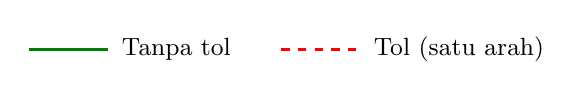
\begin{tikzpicture}[font=\small]
  \draw[green!50!black,line width=1.3pt] (0,0) -- (1.0,0);
  \node[right] at (1.05,0) {Tanpa tol};
  \draw[red,dashed,line width=1.3pt] (3.2,0) -- (4.2,0);
  \node[right] at (4.25,0) {Tol (satu arah)};
\end{tikzpicture}
\caption{Jaringan Transportasi Sederhana Kota New York dengan Tol Berarah}
\label{fig:nyc_network}
\end{figure}




\begin{casestudybox}{108{,}
\label{case:walmart-loads}000 Rute Truk Lebih Sedikit: Perencanaan Muatan Walmart}

Walmart memindahkan barang dari pusat distribusi ke sekitar 4{,}700 toko di AS menggunakan salah satu armada truk swasta terbesar di dunia. Untuk Penghargaan Franz Edelman 2023 (yang dimenangkannya), Walmart menjelaskan suatu kerangka optimisasi menyeluruh, dari desain jaringan jangka panjang hingga perutean harian dan perencanaan muatan trailer. Pada tahun fiskal 2023, sistem tersebut meniadakan 108{,}000 rute truk dan 33 juta mil perjalanan, menghemat \$91,5 juta dan mencegah emisi 98,6 juta pon CO$_2$.

\subsection*{Tantangan}
Setiap hari, setiap toko perlu menerima serangkaian pesanan. Pesanan memakai ruang trailer; truk memiliki kapasitas; toko memiliki jendela waktu pengiriman; dan setiap truk yang diberangkatkan menimbulkan biaya dan emisi. Pertanyaan harian yang menjadi inti perencanaan muatan ialah: muat pesanan ke dalam trailer sesedikit mungkin sambil tetap mematuhi kapasitas dan persyaratan pengiriman.

\subsection*{Solusi: Program Bilangan Bulat Pengepakan/Konsolidasi}
\textbf{Jenis model: pemrograman bilangan bulat untuk konsolidasi muatan dan perutean, di dalam kerangka yang lapisan strategisnya juga berupa model optimisasi. Prakiraan menjadi data masukan bagi model.}

Inti konsolidasinya, dalam bentuk sederhana:

\modelhead{Himpunan dan Parameter}
\begin{itemize}
\item Misalkan $O$ adalah himpunan pesanan untuk suatu wilayah pengiriman, dengan ukuran $q_o$ (kubikasi trailer).
\item Misalkan $T$ adalah himpunan muatan trailer (truk) yang tersedia, masing-masing dengan kapasitas $Q$.
\item Data kompatibilitas: $s_{ot} = 1$ jika pesanan $o$ dapat diangkut dengan truk $t$ (koridor rute yang sama, jendela waktu pengiriman yang layak).
\end{itemize}

\modelhead{Variabel}
\begin{itemize}
\item Misalkan $x_{ot} = 1$ jika pesanan $o$ dimuat ke truk $t$.
\item Misalkan $y_t = 1$ jika truk $t$ diberangkatkan.
\end{itemize}

\modelhead{Model}
\begin{align*}
\min \quad & \sum_{t \in T} y_t   \tag{truk yang diberangkatkan} \\
\st        & \sum_{t \in T} s_{ot}\, x_{ot} = 1 &&\quad \text{untuk semua } o \in O   \tag{setiap pesanan dikirim} \\
           & \sum_{o \in O} q_o\, x_{ot} \leq Q\, y_t &&\quad \text{untuk semua } t \in T   \tag{kapasitas; hanya menaiki truk yang diberangkatkan} \\
           & x_{ot} \leq s_{ot}, \quad x_{ot}, y_t \in \{0,1\}.
\end{align*}

Kendala kapasitas kembali menggunakan pola pengaitan Big-$M$ dengan $M = Q$. Sistem yang diterapkan menggabungkan keputusan pengepakan ini dengan perutean (toko mana yang berbagi rute) dan dengan desain jaringan strategis; makalah Edelman menjelaskan arsitektur lengkapnya.

\subsection*{Asumsi dan Penyederhanaan}
\begin{itemize}
\item Ukuran pesanan dan jendela waktu pengiriman merupakan data; dalam praktiknya, keduanya berasal dari prakiraan permintaan.
\item Model sederhana tersebut meminimumkan jumlah truk; fungsi objektif Walmart juga memperhitungkan harga per mil, sehingga konsolidasi menjadi rute yang lebih sedikit, lebih penuh, dan lebih pendek menghasilkan pengurangan 33 juta mil.
\item Perutean (urutan truk mengunjungi toko) merupakan lapisan tersendiri yang lebih sulit dan termasuk wilayah Buku 2; kotak ini menampilkan lapisan konsolidasi.
\end{itemize}

\subsection*{Implementasi dan Hasil}
Diterapkan di seluruh rantai pasok Walmart di AS: 108{,}000 rute dan 33 juta mil ditiadakan pada FY2023, penghematan \$91,5 juta, dan pencegahan emisi 98,6 juta pon CO$_2$. Pemenang Penghargaan Franz Edelman INFORMS 2023.

\subsection*{Referensi}
\begin{itemize}
\item ``Optimizing Walmart's Supply Chain from Strategy to Execution.'' \emph{INFORMS Journal on Applied Analytics} 54(1), 5--19, 2024. \url{https://doi.org/10.1287/inte.2023.0093}
\end{itemize}
\end{casestudybox}

\subsection{Kendala Salah Satu}
\label{subsec:either-or}
Teknik Big-M pada subbagian sebelumnya mengaktifkan satu kendala. Keadaan yang sangat terkait terjadi ketika kita memiliki dua kendala dan memerlukan \emph{setidaknya satu} di antaranya berlaku: suatu \emph{atau inklusif}. Misalnya, sebuah kiriman mungkin harus tiba sebelum tenggat pagi atau setelah pembukaan sore, atau anggaran harus dipenuhi dalam setidaknya satu dari dua mata uang. Triknya adalah menggunakan satu variabel biner untuk menentukan kendala \emph{mana} yang diterapkan, dan sepasang kendala Big-M untuk merelaksasi kendala yang tidak dipilih.
\begin{general}{Salah Satu}{}{}

\begin{equation}
\text{Salah satu dari } \ \ \ a^\top x \leq b\ \  \text{ atau } \ \  c^\top x \leq d \ \ \text{berlaku}
\end{equation}
dapat dimodelkan sebagai
\begin{equation}
\begin{split}
a^\top x - b &\leq M_1 \delta\\
c^\top x - d &\leq M_2 (1-\delta)\\
\delta &\in \{0,1\},
\end{split}
\end{equation}
dengan $M_1$ sebagai batas atas $a^\top x - b$ dan $M_2$ sebagai batas atas $c^\top x - d$.
\end{general}

\paragraph{Interpretasi.}
\begin{itemize}
    \item Jika \(\delta = 0\), kendala pertama menjadi \(a^\top x \leq b\), sedangkan kendala kedua menjadi \(c^\top x \leq d + M_2\), yang dipenuhi secara trivial jika \(M_2\) cukup besar.
    \item Jika \(\delta = 1\), kendala kedua menjadi \(c^\top x \leq d\), sedangkan kendala pertama direlaksasi menjadi \(a^\top x \leq b + M_1\).
\end{itemize}
Dalam kedua keadaan tersebut, setidaknya satu dari dua kendala asli diterapkan; variabel biner $\delta$ hanya menentukan kendala mana yang dipilih.

Sekarang kita terapkan pola ini pada sebuah contoh kecil.

\begin{example}{Bus atau Mobil}{}
Untuk mengantar para siswa ke pertandingan sepak bola, kita memerlukan setidaknya $2$ bus atau setidaknya $10$ mobil.
\begin{itemize}
\item Misalkan $x$ adalah jumlah bus yang kita miliki dan
\item misalkan $y$ adalah jumlah mobil yang kita miliki.
\end{itemize}
Kita hendak menerapkan $x \geq 2$ atau $y \geq 10$. Dengan menuliskannya dalam bentuk yang digunakan di atas, kita memerlukan $-x \leq -2$ atau $-y \leq -10$. Karena $x, y \geq 0$, kita dapat mengambil $M_1 = 2$ sebagai batas atas $-x - (-2) = 2 - x$ dan $M_2 = 10$ sebagai batas atas $10 - y$. Pola tersebut menghasilkan
\begin{equation}
\begin{split}
2 - x &\leq 2\delta\\
10 - y &\leq 10 (1-\delta)\\
\delta &\in \{0,1\},
\end{split}
\end{equation}
yang menyederhana menjadi $x \geq 2(1-\delta)$ dan $y \geq 10\delta$. Jika $\delta = 0$, kita harus memiliki setidaknya $2$ bus; jika $\delta = 1$, kita harus memiliki setidaknya $10$ mobil.
\end{example}

\paragraph{Memilih Nilai Big-M.}
\label{par:choosing-big-M}
Konstanta \(M_1\) dan \(M_2\) masing-masing harus dipilih sebagai batas atas yang sah bagi ekspresi \(a^\top x - b\) dan \(c^\top x - d\) pada daerah layak. Nilai yang terlalu besar dapat melemahkan relaksasi LP dan menyebabkan ketidakstabilan numerik, sehingga penetapan batas secara cermat disarankan apabila memungkinkan. Pada contoh di atas, batas $M_1 = 2$ dan $M_2 = 10$ adalah batas seketat mungkin.

\paragraph{Kasus Penggunaan.}
Kendala salah satu muncul secara alami dalam masalah dengan keputusan bersyarat, seperti:
\begin{itemize}
    \item Jika sebuah mesin digunakan, salah satu dari kendala energi tertentu atau kendala keselamatan harus dipenuhi.
    \item Dalam perencanaan fasilitas, suatu lokasi harus dibangun dengan salah satu dari dua konfigurasi.
    \item Dalam model sepenggal, variabel harus berada dalam salah satu dari dua daerah layak.
\end{itemize}
Kita akan melihat penerapan penting gagasan ini, dengan lebih dari dua kendala dalam disjungsi, ketika mempelajari masalah pengepakan 2D pada Bagian~\ref{subsec:multi-term-disjunction}.
\subsection{Implikasi Jika--maka - Arah Sebaliknya}
Misalkan kita ingin memodelkan kenyataan bahwa jika paling banyak 10 mahasiswa mengikuti mata kuliah ini, maka kita harus berpindah ke ruang kelas yang lebih kecil.

Misalkan $x_i \in \{0,1\}$ bernilai 1 jika mahasiswa $i$ mengikuti mata kuliah tersebut. Misalkan $\delta \in \{0,1\}$ bernilai 1 jika kita perlu berpindah ke ruang kelas yang lebih kecil.

Jadi, kita ingin memodelkan
\begin{quote}
Jika $$
\sum_{i \in I} x_i \leq 10
$$
maka
$$
\delta = 1.
$$
\end{quote}

Dengan menggunakan pola di bawah ini dengan $b = 10$, $\epsilon = 1$ (datanya berupa bilangan bulat), dan batas bawah $m = -10$ bagi $\sum_{i \in I} x_i - 10$, kita dapat memodelkannya sebagai
\begin{equation}
\sum_{i \in I} x_i \geq 10 + 1(1-\delta) + (-10)\delta = 11(1 - \delta).
\end{equation}
Jika $\delta = 0$, kendala memaksa setidaknya $11$ mahasiswa; secara ekuivalen (melalui kontraposisi), setiap kali $10$ mahasiswa atau kurang hadir, model harus menetapkan $\delta = 1$.


\begin{general}{Jika pertidaksamaan, maka indikator}{}
Misalkan $m$ adalah batas bawah kuantitas $a^\top x - b$ dan $\epsilon$ adalah bilangan kecil yang menjadi batas galat ketika memeriksa apakah suatu pertidaksamaan dilanggar. \textbf{Jika data $a,b$ berupa bilangan bulat dan $x$ juga bilangan bulat, kita dapat mengambil $\epsilon = 1$.}

Sekarang
\begin{equation}
\text{Jika } \ \ a^\top x \leq b  \ \ \text{maka}\ \ \delta = 1
\end{equation}
dapat dimodelkan sebagai
\begin{equation}
a^\top x -b  \geq  \epsilon(1-\delta) + m \delta.
\end{equation}
\end{general}



\begin{proof}Sekarang kita membuktikan pernyataan di atas.

Cara sederhana untuk memahami kendala ini adalah mempertimbangkan \emph{kontraposisi} pernyataan jika--maka yang hendak dimodelkan. Kontraposisi tersebut menyatakan bahwa
\begin{equation}
\text{Jika $\delta = 0$, maka $a^\top x - b > 0$.}
\end{equation}
Untuk menunjukkan kontraposisi tersebut, kita tetapkan $\delta = 0$. Pertidaksamaannya kemudian menjadi
$$
a^\top x - b \geq \epsilon(1-0) + m0 = \epsilon > 0.
$$
Dengan demikian, kontraposisinya berlaku.

\textbf{Jika kita justru menginginkan bukti langsung:}

Kasus 1: Misalkan $a^\top x \leq b$. Maka $0 \geq a^\top x - b$, yang menyiratkan bahwa
$$
\delta(a^\top x - b) \geq a^\top x - b
$$
Oleh karena itu
$$
\delta(a^\top x - b) \geq \epsilon(1-\delta) + m \delta
$$
Setelah disusun ulang
$$
\delta(a^\top x - b - m) \geq \epsilon(1-\delta)
$$
Karena $a^\top x - b - m \geq 0$ dan $\epsilon > 0$, satu-satunya pilihan yang layak adalah $\delta = 1$.


Kasus 2: Misalkan $a^\top x > b$. Berdasarkan pemilihan $\epsilon$, hal ini menyiratkan $a^\top x - b \geq \epsilon$, sehingga pertidaksamaan berlaku untuk $\delta = 0$. Karena $a^\top x - b \geq m$ juga berlaku, pertidaksamaan tersebut berlaku pula untuk $\delta = 1$. Jadi, kedua pilihan $\delta$ layak, sebagaimana mestinya.
\end{proof}

Banyak kombinasi lain dari pernyataan jika--maka dirangkum dalam tabel berikut:
\begin{table}
\begin{center}
\begin{tabular}{|c|c|}
\hline
\textbf{Implikasi} & \textbf{Kendala}\\
\hline
Jika $\delta = 0$, maka $a^\top x \leq b$ & $a^\top x \leq b + M \delta$\\
Jika $a^\top x \leq b$, maka $\delta = 1$ & $a^\top x \geq m \delta + \epsilon(1-\delta)$\\
\hline
\end{tabular}
\end{center}
\caption{Daftar singkat: model jika--maka dengan kendala dan variabel biner. Di sini $M$ dan $m$ adalah batas atas dan bawah bagi $a^\top x - b$, sedangkan $\epsilon$ adalah bilangan kecil sedemikian sehingga jika $a^\top x > b$, maka $a^\top x \geq b + \epsilon$.}
\end{table}
Kedua implikasi ini dapat digunakan untuk menurunkan daftar implikasi yang lebih panjang berikut.

\begin{table}
\begin{center}
\begin{tabular}{|c|c|}
\hline
\textbf{Implikasi} & \textbf{Kendala}\\
\hline
Jika $\delta = 0$, maka $a^\top x \leq b$ & $a^\top x \leq b + M \delta$\\
Jika $\delta = 0$, maka $a^\top x \geq b$ & $a^\top x \geq b + m \delta$\\
Jika $\delta = 1$, maka $a^\top x \leq b$ & $a^\top x \leq b + M (1-\delta)$\\
Jika $\delta = 1$, maka $a^\top x \geq b$ & $a^\top x \geq b + m (1-\delta)$\\
Jika $a^\top x \leq b$, maka $\delta = 1$ & $a^\top x \geq b + m \delta + \epsilon(1-\delta)$\\
Jika $a^\top x \geq b$, maka $\delta = 1$ & $a^\top x \leq b + M \delta - \epsilon(1-\delta)$\\
Jika $a^\top x \leq b$, maka $\delta = 0$ & $a^\top x \geq b + m (1-\delta) + \epsilon \delta$\\
Jika $a^\top x \geq b$, maka $\delta = 0$ & $a^\top x \leq b + M (1-\delta) - \epsilon \delta$\\
\hline
\end{tabular}
\end{center}
\caption{Daftar panjang: model jika--maka dengan kendala dan variabel biner. Di sini $M$ dan $m$ adalah batas atas dan bawah bagi $a^\top x - b$, sedangkan $\epsilon$ adalah bilangan kecil sedemikian sehingga jika $a^\top x > b$, maka $a^\top x \geq b + \epsilon$.}
\end{table}
Terakhir, jika Anda bersikeras menginginkan kesesuaian persis, yaitu, ``$\delta = 0 $ jika dan hanya jika $a^\top x \leq b$'', Anda cukup menyertakan kedua kendala untuk ``jika $\delta = 0 $, maka $a^\top x \leq b$'' dan ``jika $a^\top x \leq b$, maka $\delta = 0 $''. Meskipun banyak masalah mungkin dinyatakan seolah-olah memerlukan ``jika dan hanya jika'', sering kali kedua kendala tidak perlu digunakan karena fungsi objektif dalam masalah secara alami mencegah salah satu keadaan tersebut terjadi.

Sebagai contoh, jika kita ingin menambahkan variabel biner $\delta$ yang berarti
$$
\begin{cases}
\delta = 0 \text{ menyiratkan }  a^\top x \leq b\\
\delta = 1  \text{ Jika tidak}
\end{cases}
$$
Jika $\delta = 1$ tidak memengaruhi bagian lain dari masalah optimisasi, penambahan kendala mengenai $\delta = 1$ tidak diperlukan. Oleh karena itu, dalam skenario ini biasanya kita hanya perlu menambahkan kendala $a^\top x \leq b + M \delta$.

\subsection{Disjungsi Multisuku dengan Penerapan pada Pengepakan 2D}
\label{subsec:multi-term-disjunction}

%\section{Disjungsi $k$-dari-$n$ Terampat}
Disjungsi merupakan perampatan pernyataan ``atau''. Misalkan kita memiliki $n$ kendala
	$$
	\mathbf{a}_1^\top\mathbf{x} \leq b_1, \quad \mathbf{a}_2^\top\mathbf{x} \leq b_2, \quad\dots, \quad \mathbf{a}_n^\top\mathbf{x} \leq b_n
	$$
dan kita hendak menerapkan paling sedikit $k$ di antaranya. Hal ini dapat dicapai secara linier dengan memperkenalkan variabel indikator biner baru $\delta_i$ bagi setiap kendala disjungtif $i \in \{1,\dots,n\}$:
	\begin{align*}
	\mathbf{a}_1^\top\mathbf{x} &\leq b_1+M(1-\delta_1) \\
	\mathbf{a}_2^\top\mathbf{x} &\leq b_2+M(1-\delta_2) \\
								&\vdots 				\\
	\mathbf{a}_n^\top\mathbf{x} &\leq b_n+M(1-\delta_n) \\
	\sum_{i=1}^n\delta_i &\geq k
	\end{align*}
Jika $\delta_i = 1$, kendala disjungtif $i^\text{th}$ diterapkan secara aktif. Kendala terakhir $\left(\sum_{i=1}^n\delta_i \geq k\right)$ memastikan bahwa setidaknya $k$ kendala aktif.

\subsubsection{Masalah Pengepakan Strip}
Misalkan kita memiliki koleksi persegi panjang $I$ dan strip dua dimensi dengan lebar $W$ dan tinggi tak terhingga. Setiap persegi panjang $i \in I$ memiliki lebar $w_i$ dan
tinggi $h_i$, dan kita hendak mengepak persegi panjang ke dalam strip sedemikian sehingga tinggi keseluruhan \eqref{mod:StripPackingObj-simple} diminimumkan, lebar keseluruhan \eqref{mod:StripPackingWidth-simple} kurang dari $W$, dan tidak ada persegi panjang yang saling tumpang-tindih \eqref{mod:StripPackingOverlap-simple}. Lihat Gambar \ref{fig:StripPacking} sebagai contoh: Gambar \ref{fig:StripPacking-PackStrip} menunjukkan persegi panjang yang akan dikemas, dan Gambar \ref{fig:StripPacking-MinHeight} menunjukkan suatu pengepakan dengan tinggi keseluruhan $H$ yang hendak diminimumkan.
	\begin{figure}[h!]
	\begin{subfigure}[b]{.6\textwidth}
	\centering
	
\includegraphics[height=.4\textheight]{optimization/figures/figures-static/StripPacking0}
	\caption{Kemas persegi panjang ke dalam strip}
	\label{fig:StripPacking-PackStrip}
	\end{subfigure}
	\hfill
	\begin{subfigure}[b]{.3\textwidth}
	\centering
	
\includegraphics[height=.4\textheight]{optimization/figures/figures-static/StripPacking1}
	\caption{Minimumkan tinggi keseluruhan $H$.}
	\label{fig:StripPacking-MinHeight}
	\end{subfigure}
	\caption{Contoh Masalah Pengepakan Strip}
	\label{fig:StripPacking}
	\end{figure}

Misalkan $(x_i,y_i)$ menyatakan posisi sudut kiri bawah setiap persegi panjang $i \in I$. Kendala tumpang-tindih \eqref{mod:StripPackingOverlap-simple} merupakan bagian tersulit. Pertimbangkan sepasang persegi panjang $i$ dan $j$: persegi panjang $j$ terletak sepenuhnya di sebelah kiri persegi panjang $i$ jika $x_i$ memiliki nilai lebih besar daripada $x_j+w_j$. Artinya, jika $x_j + w_j \leq x_i$. Di sisi lain, jika $y_j \geq y_i+h_i$, maka persegi panjang $j$ terletak sepenuhnya di atas persegi panjang $i$. Jika salah satu kendala ini dipenuhi, maka persegi panjang $i$ dan $j$ tidak tumpang-tindih. Kita juga dapat menempatkan $i$ di atas atau di sebelah kanan $j$. Hal ini menghasilkan empat kendala yang setidaknya salah satunya harus dipenuhi. Modelnya dapat dipahami sebagai berikut:

	\begin{subequations}
	\begin{alignat}{4}
	\text{Minimumkan}& \quad & \mathclap{\hspace{-69pt} \max_{i\in I}\{y_i+h_i\}} 	\label{mod:StripPackingObj-simple}\\
		\st & 	   & \max_{i\in I}\{x_i+w_i\} &\leq W 						\label{mod:StripPackingWidth-simple}\\
				   &	   & \mathclap{\hspace{111pt} \left.\begin{aligned}
				   		x_i+w_i &\leq x_j \\
				   		x_j+w_j &\leq x_i \\
				   		y_i+h_i &\leq y_j \\
				   		y_j+h_j &\leq y_i
				   	\end{aligned}\right\} \parbox{110pt}{Setidaknya satu di antaranya untuk setiap pasangan persegi panjang berbeda $i,j \in I$}} \label{mod:StripPackingOverlap-simple} \\
			   	   &	   & x_i,y_i &\geq 0		&\qquad& & &\forall\ i\in I
	\end{alignat}
	\end{subequations}
Kendala \eqref{mod:StripPackingOverlap-simple} adalah himpunan empat kendala \textit{disjungtif}. Kendala ini dapat dinyatakan secara linier dengan memperkenalkan variabel indikator biner baru $\delta_{ijk}$ untuk setiap kendala disjungtif dalam \eqref{mod:StripPackingOverlap-simple}:
	\begin{alignat}{4}
	\text{Minimumkan}& \quad & \mathclap{\hspace{-53pt} H}	\nonumber\\
		\st & 	   & y_i+h_i &\leq H						&\qquad& & &\forall\ i\in I		\tag{\ref{mod:StripPackingObj-simple}}	\\
				   & 	   & x_i+w_i &\leq W						&\qquad& & &\forall\ i\in I		\tag{\ref{mod:StripPackingWidth-simple}}\\
				   &	   & x_i+w_i &\leq x_j+M(1-\delta_{ij1}) 	&\qquad& & &\forall\ i,j\in I:\ i>j	\nonumber \\
				   &	   & x_j+w_j &\leq x_i+M(1-\delta_{ij2}) 	&\qquad& & &\forall\ i,j\in I:\ i>j	\nonumber \\
				   &	   & y_i+h_i &\leq y_j+M(1-\delta_{ij3}) 	&\qquad& & &\forall\ i,j\in I:\ i>j	\tag{\ref{mod:StripPackingOverlap-simple}}\\
				   &	   & y_j+h_j &\leq y_i+M(1-\delta_{ij4}) 	&\qquad& & &\forall\ i,j\in I:\ i>j	\nonumber \\
				   &	   & \sum_{k=1}^4\delta_{ijk} & \geq 1	 	&\qquad& & &\forall\ i,j\in I:\ i>j	\nonumber \\
				   &	   & x_i,y_i &\geq 0		&\qquad& & &\forall\ i\in I							\nonumber \\
				   &	   & \boldsymbol{\delta}_{ij} &\in\{0,1\}^4	&\qquad& & &\forall\ i,j\in I:\ i>j	\nonumber 
	\end{alignat}
Jika $\delta_{ijk} = 1$, kendala disjungtif $k^\text{th}$ diterapkan secara aktif. Kendala terakhir $\left(\sum_{k=1}^4\delta_{ijk} \geq 1\right)$ memastikan bahwa setidaknya satu kendala aktif. Solusi optimal untuk contoh tersebut diberikan pada Gambar \ref{fig:StripPacking-Opt}; solusi itu ditemukan menggunakan GurobiPy.
	\begin{figure}[h!]
	\centering
	
\includegraphics[height=.4\textheight]{optimization/figures/figures-static/StripPacking2}
	\caption{Solusi optimal untuk contoh pengepakan strip.}
	\label{fig:StripPacking-Opt}
	\end{figure}

Masalah ini dianggap NP-Hard kuat.






\subsection{Kendala SOS1}
Trik pemodelan sejauh ini dalam bagian ini dibangun secara manual dari variabel biner dan kendala Big-M. Namun, struktur logis tertentu begitu sering muncul sehingga pemecah modern menerimanya secara langsung sebagai \emph{himpunan terurut khusus} (special ordered sets, SOS). Mendeklarasikan kendala SOS memberi tahu pemecah mengenai struktur tersebut secara eksplisit, yang sekaligus menyederhanakan model yang Anda tulis dan memungkinkan pemecah menggunakan aturan percabangan khusus.
\begin{definition}{Himpunan Terurut Khusus Tipe 1 (SOS1)}
Kendala Himpunan Terurut Khusus tipe 1 (SOS1) pada suatu vektor menunjukkan bahwa \emph{paling banyak satu unsur vektor dapat bernilai taknol}.
\end{definition}
Kendala SOS1 muncul setiap kali suatu himpunan pilihan bersifat saling eksklusif: memilih satu pemasok dari beberapa pemasok, mengoperasikan mesin dalam salah satu dari beberapa modus, atau menetapkan kiriman ke salah satu dari beberapa rute. Jika setiap $x_i$ memiliki batas atas $U_i$, kita dapat memodelkannya sendiri dengan memperkenalkan variabel biner $z_i$ untuk setiap $x_i$ dan menuliskan $x_i \leq U_i z_i$ bersama dengan $\sum_i z_i \leq 1$. Mendeklarasikan kendala SOS1 menghasilkan efek yang sama hanya dengan satu baris kode dan tanpa variabel tambahan.

Contoh kecil berikut sengaja dibuat sederhana: tujuannya bukan masalah optimisasi itu sendiri, melainkan melihat kedua gaya pemodelan secara berdampingan dalam kode.

\begin{examplewithcode}{Kendala SOS1}{\href{https://github.com/open-optimization/open-optimization-or-examples/blob/master/nonlinear-programming/Gurobi-SOS-Examples.ipynb}{Gurobipy}}
\label{example:sos1}
Selesaikan masalah optimisasi berikut: \[\begin{aligned}
\text{maksimumkan}\quad & 3x_1 + 4x_2 + x_3 + 5x_4 \\
\st \quad & 0 \le x_i \le 5 \\
& \text{paling banyak satu dari $x_i$ dapat bernilai taknol}
\end{aligned}\]
Karena hanya satu variabel yang boleh bernilai taknol, pilihan terbaik adalah mendorong variabel dengan koefisien objektif terbesar, $x_4$, sampai ke batas atasnya: solusi optimalnya adalah $x_4 = 5$ dengan nilai $25$.
\end{examplewithcode}
\subsection{Kendala SOS2}
\begin{definition}{Himpunan Terurut Khusus Tipe 2 (SOS2)}{}
Kendala \emph{Himpunan Terurut Khusus Tipe 2 (SOS2)} pada suatu vektor menunjukkan bahwa \emph{paling banyak dua unsur vektor dapat bernilai taknol DAN unsur taknol tersebut harus muncul secara berurutan}.
\end{definition}
Sekilas, kondisi ini tampak ganjil untuk diperlakukan secara khusus, tetapi inilah tepatnya yang diperlukan untuk memodelkan \emph{fungsi linier sepenggal}: sebuah titik pada kurva linier sepenggal terletak pada satu segmen, sehingga dapat ditulis sebagai rata-rata berbobot dari dua titik patah \emph{berurutan} pada ujung segmen tersebut. Kita mengembangkan penerapan itu dalam subbagian berikutnya; di sini, kita terlebih dahulu membiasakan diri dengan kendala tersebut.

Contoh di bawah hanya mengubah contoh SOS1 dalam satu hal (dua nilai taknol yang berurutan sekarang diperbolehkan), sehingga kedua contoh mudah dibandingkan. Seperti sebelumnya, kode pendamping menampilkan formulasi variabel biner dan deklarasi SOS2 satu baris.

\begin{examplewithcode}{SOS2}{\href{https://github.com/open-optimization/open-optimization-or-examples/blob/master/nonlinear-programming/Gurobi-SOS-Examples.ipynb}{Gurobipy}}
\label{example:SOS2}
Selesaikan masalah optimisasi berikut: \[\begin{aligned}
\text{maksimumkan}\quad & 3x_1 + 4x_2 + x_3 + 5x_4 \\
\st \quad & 0 \le x_i \le 5 \\
& \text{paling banyak dua dari $x_i$ dapat bernilai taknol} \\
& \text{dan $x_i$ taknol harus berurutan}
\end{aligned}\]
Pasangan variabel berurutan adalah $(x_1,x_2)$, $(x_2,x_3)$, dan $(x_3,x_4)$. Dengan membandingkan koefisien objektif, pasangan terbaik adalah $(x_1, x_2)$ pada $x_1 = x_2 = 5$, yang memberikan nilai $(3+4)\cdot 5 = 35$. Perhatikan bahwa solusi SOS1 $x_4=5$ saja hanya memberikan $25$.
\end{examplewithcode}

\subsection{Fungsi Linier Sepenggal dengan Kendala SOS2}
\label{subsec:pwl-sos2}
\begin{examplewithcode}{Fungsi Linier Sepenggal}{\href{https://github.com/open-optimization/open-optimization-or-examples/blob/master/nonlinear-programming/Gurobi-SOS-Examples.ipynb}{Gurobipy}}
\label{example:pwl}
Pertimbangkan fungsi linier sepenggal
 $c(x)$ yang diberikan oleh
$$
c(x) = 
\begin{cases}
25x  & \text{ jika } 0 \leq x \leq 5\\
20x + 25 & \text{ jika } 5 \leq x \leq 10\\
15x + 75 & \text{ jika } 10 \leq x \leq 15
\end{cases}
$$
\begin{center}
% Versi lokal yang dapat diedit menggantikan raster sumber berlabel Inggris.
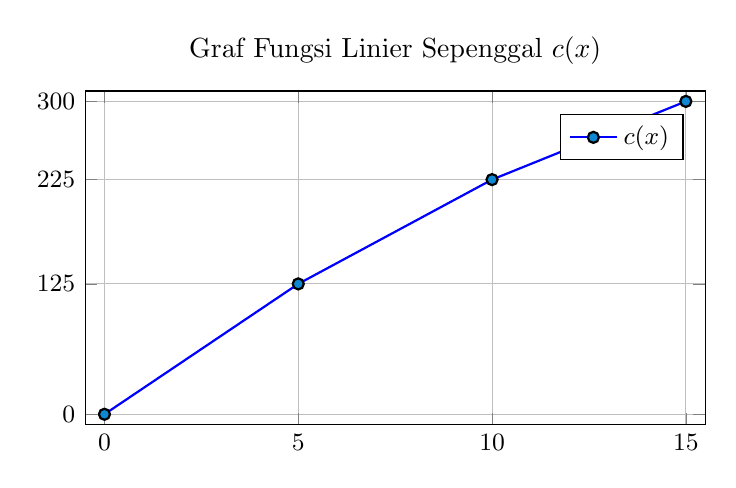
\begin{tikzpicture}
\begin{axis}[
  width=0.78\textwidth,
  height=0.48\textwidth,
  title={Graf Fungsi Linier Sepenggal $c(x)$},
  xmin=-0.5,
  xmax=15.5,
  ymin=-10,
  ymax=310,
  xtick={0,5,10,15},
  ytick={0,125,225,300},
  grid=major,
  axis line style={black},
  tick label style={font=\small},
  title style={font=\normalsize},
  legend style={
    at={(0.965,0.93)},
    anchor=north east,
    draw=black,
    fill=white,
    font=\small
  }
]
\addplot[
  blue,
  thick,
  mark=*,
  mark options={fill=cyan!70!blue,draw=black}
] coordinates {(0,0) (5,125) (10,225) (15,300)};
\addlegendentry{$c(x)$}
\end{axis}
\end{tikzpicture}
\par\captionof{figure}{Fungsi linier sepenggal.}\label{fig:pwl-plot}% fig-num-auto

\end{center}
%Lihat \refincludefigurestatic[scale = 0.35]{pwl-plot.png}.

Kita akan menggunakan pemrograman bilangan bulat untuk mendeskripsikan fungsi ini. Kita akan menetapkan $x = a$, lalu program bilangan bulat akan menetapkan nilai $y$ menjadi $c(a)$.
\begin{align*}
\min \quad & 0 \\
\st        & x = 5 z_{2} +10 z_{3} + 15 z_{4} \\
 & y = 125 z_{2} + 225 z_{3} + 300 z_{4} \\
 & z_{1} + z_{2} + z_{3} + z_{4} = 1 \\
 & SOS2: \{z_1, z_2, z_3, z_4\} \\
 & 0 \leq z_{i} \leq 1 &&\quad \text{untuk semua } i \in \{1,2,3,4\} \\
 & x = a \\
\end{align*}

\end{examplewithcode}

\begin{examplewithcode}{Penerapan Fungsi Linier Sepenggal}{\href{https://github.com/open-optimization/open-optimization-or-examples/blob/master/nonlinear-programming/Gurobi-SOS-Examples.ipynb}{Gurobipy}}
\label{example:pwl-application}
Pertimbangkan masalah optimisasi berikut yang fungsi objektifnya mencakup suku $c(x)$, dengan $c(x)$ sebagai fungsi linier sepenggal yang dijelaskan dalam \nameref{example:pwl}:
\begin{align}
\max \quad & z = 12x_{11} + 12x_{21} + 14x_{12} + 14x_{22} - c(x) \\
\st        & x_{11} + x_{12} \leq x + 5 \\
& x_{21} + x_{22} \leq 10 \\
& 0.5 x_{11} - 0.5x_{21} \geq 0 \\
& 0.4 x_{12} - 0.6 x_{22} \geq 0 \\
& x_{ij} \geq 0 \\
& 0 \leq x \leq 15
\end{align}

Dengan fungsi linier sepenggal tersebut, kita dapat memodelkan seluruh masalah secara eksplisit sebagai program linier bilangan bulat campuran.

 \begin{equation}
 \begin{array}{rrlr}
 \max\quad & 12 X_{1,1} + 12 X_{2,1} + 14 X_{1,2} + 14 X_{2,2} - y\\
\st \quad & x - 5 z_{2} - 10 z_{3} - 15 z_{4} &= 0\\
 & y - 125 z_{2} - 225 z_{3} - 300 z_{4} &= 0\\
 & z_{1} + z_{2} + z_{3} + z_{4} &= 1\\
 & X_{1,1} + X_{1,2} - x &\leq 5\\
 & X_{2,1} + X_{2,2} &\leq 10\\
 & 0.5 X_{1,1} - 0.5 X_{2,1} &\geq 0\\
 & 0.4 X_{1,2} - 0.6 X_{2,2} &\geq 0\\
 & SOS2: \{z_1, z_2, z_3, z_4\}\\
 & X_{i,j} &\geq 0 &\quad\forall i \in \{1,2\}, j \in \{1,2\}\\
 & 0 \leq z_{i} &\leq 1 &\quad\forall i \in \{1,2,3,4\}\\
 & 0 \leq x &\leq 15\\
 & y & \text{ bebas} \\
\end{array}
\end{equation}
\end{examplewithcode}


\subsubsection{SOS2 dengan Variabel Biner}

Jika pemecah tidak mendukung kendala SOS2 secara langsung, kita dapat menerapkan kondisi yang sama dengan variabel biner. Pola untuk fungsi linier sepenggal $f$ dengan titik patah $a_1 < a_2 < \dots < a_k$ adalah:
\begin{itemize}
\item Tuliskan pasangan titik patah dan nilai fungsi $(a_i, f(a_i))$.
\item Definisikan variabel biner $z_i$ yang menunjukkan apakah $x$ berada dalam interval $[a_i, a_{i+1}]$.
\item Definisikan pengali $\lambda_i$ sedemikian sehingga $x$ merupakan kombinasi dari $a_i$, dan karena itu keluaran $y = f(x)$ merupakan kombinasi dari $f(a_i)$.
\item Batasi agar paling banyak 2 dari $\lambda_i$ bernilai taknol dan kedua nilai tersebut berurutan.

\end{itemize}

\begin{align*}
\min \quad & \sum_{i=1}^k \lambda_i f(a_i) \\
\st        & \sum_{i=1}^k \lambda_i = 1 \\
& x = \sum_{i=1}^k \lambda_i a_i \\
& \sum_{i=1}^{k-1} z_i = 1 \\
& \lambda_1 \leq z_1 \\
& \lambda_i \leq z_{i-1} + z_{i} &&\quad \text{untuk semua } i=2, \dots, k-1, \\
& \lambda_k \leq z_{k-1} \\
& \lambda_i \geq 0, z_i \in \{0,1\}.
\end{align*}

Di sini variabel biner $z_i$ memilih segmen $i$: kendala $\sum_{i=1}^{k-1} z_i = 1$ memilih tepat satu interval $[a_i, a_{i+1}]$, lalu kendala $\lambda_j \leq z_{j-1} + z_j$ memaksa $\lambda_j = 0$ untuk setiap indeks $j$ di luar $\{i, i+1\}$. Hanya $\lambda_i$ dan $\lambda_{i+1}$ yang dapat bernilai taknol, yang tepat merupakan kondisi SOS2.

\subsection{Memaksimumkan Nilai Minimum}
Jika kendalanya dapat bersifat umum, kita akan menulis $x \in X$ untuk mendefinisikan kendala umum. Misalnya, kita dapat memiliki $X = \{ x \in \R^n : Ax \leq b\}$ atau $X  = \{ x \in \R^n : Ax \leq b, x \in \Z^n\}$ atau berbagai kemungkinan lain.


Pertimbangkan masalah

\begin{align*}
\max   \quad & \min \{x_1, \dots, x_n\}\\
\text{ dengan syarat } \quad &  x \in X
\end{align*}
Keberadaan nilai minimum di bagian dalam kurang praktis. Untuk menghilangkannya, kita cukup mendefinisikan variabel baru $y$ dan menerapkan $y \leq x_i$, lalu memaksimumkan $y$. Karena kita memaksimumkan $y$, variabel itu akan mengambil nilai $x_i$ terkecil. Dengan demikian, kita dapat merumuskan ulang masalahnya sebagai

\begin{align*}
\max\quad    & y\\
\text{ dengan syarat } \quad  & y \leq x_i \ \text{ untuk }\  i=1, \dots, n \\
&  x \in X
\end{align*}


\subsection{Merelaksasi Kendala Kesamaan (Nonlinier)}

Ada sejumlah skenario ketika kendala dapat direlaksasi tanpa mengorbankan solusi optimal masalah Anda. Serupa dengan memaksimumkan nilai minimum, jika berdasarkan fungsi objektif kita mengetahui bahwa kendala tertentu akan aktif pada solusi optimal, kita dapat merelaksasi kesamaan menjadi pertidaksamaan. Sebagai contoh,
\begin{align*}
\max   \quad &x_1 + x_2 +  \dots + x_n\\
\text{ dengan syarat } \quad &  x_i = y_i^2 + z_i^2 \text{ untuk } i=1, \dots, n
\end{align*}
Karena fungsi objektif mendorong setiap $x_i$ ke atas, kita dapat merelaksasi kesamaan menjadi
\begin{align*}
\max   \quad &x_1 + x_2 +  \dots + x_n\\
\text{ dengan syarat } \quad &  x_i \leq y_i^2 + z_i^2 \text{ untuk } i=1, \dots, n
\end{align*}
Pada setiap solusi optimal masalah yang direlaksasi, setiap $x_i$ sebesar yang diperbolehkan kendalanya, sehingga $x_i = y_i^2 + z_i^2$ berlaku dan solusi optimal tidak berubah. Trik ini sah setiap kali dorongan fungsi objektif memaksa pertidaksamaan yang direlaksasi menjadi aktif pada optimum. Perhatikan bahwa arahnya penting: merelaksasi menjadi $x_i \geq y_i^2 + z_i^2$ justru akan memungkinkan $x_i$ bertambah tanpa batas.






%
%\subsection{Menghubungkan dengan variabel kontinu}
%
%Misalkan $x_i \geq 0$ dan $y_i \in \{0,1\}$ untuk semua $i=1, \dots, n$.
%
%\begin{enumerate}
%\item Jika $x_i > 0$, maka $y_i = 1$.
%\begin{equation}
%x_i \leq M y_i
%\end{equation}
%dengan $M$ sebagai batas atas yang cukup besar bagi variabel $x_i$.
%\item Jika $x_i = 0$, maka $y_i = 0$.\\
%Hal ini lebih sulit dimodelkan! Sebagai alternatif, kita mencoba memodelkan "jika $x_i$ cukup kecil, maka $y_i = 0$. Misalnya, jika $x_i \leq 0.0000001$, maka $y_i = 0$.
%Hal ini dapat dimodelkan sebagai
%\begin{equation}
%x_i - 0.0000001 \geq y_i -1.
%\end{equation}
%\item Jika $y_i = 1$, maka $x_i \geq 5$
%\begin{equation}
%5y_i \leq x_i.
%\end{equation}
%\end{enumerate}

\subsection{Memodelkan Nilai Mutlak Eksak}
Dalam banyak formulasi, kita perlu menerapkan kendala $|x| = t$ dengan $t \geq 0$.
Perhatikan bahwa versi pertidaksamaan $|x| \leq t$ ekuivalen dengan pasangan kendala linier $-t \leq x \leq t$ dan tidak memerlukan variabel bilangan bulat.
Namun, \emph{kesamaan} $|x| = t$ mendefinisikan himpunan noncembung (gabungan dari $x = t$ dan $x = -t$), sehingga tidak dapat dimodelkan hanya dengan kendala linier.

Untuk menanganinya, uraikan $x$ menjadi bagian positif dan negatifnya: tuliskan $x = x^+ - x^-$ dengan $x^+, x^- \geq 0$.
Kemudian $|x| = x^+ + x^-$ asalkan $x^+$ dan $x^-$ tidak positif secara bersamaan.
Kita menerapkan kondisi komplementaritas ini dengan variabel biner $z \in \{0,1\}$ dan konstanta $M$ yang cukup besar (batas atas $|x|$ dalam konteks masalah):
\begin{align}
x &= x^+ - x^-, \notag\\
t &= x^+ + x^-, \notag\\
x^+ &\leq Mz, \label{eq:abs-pos-bound}\\
x^- &\leq M(1-z), \label{eq:abs-neg-bound}\\
x^+, x^- &\geq 0, \quad z \in \{0,1\}. \notag
\end{align}
Ketika $z=1$, kendala~\eqref{eq:abs-neg-bound} memaksa $x^- = 0$, sehingga $x = x^+ \geq 0$.
Ketika $z=0$, kendala~\eqref{eq:abs-pos-bound} memaksa $x^+ = 0$, sehingga $x = -x^- \leq 0$.
Pada kedua kasus, $t = |x|$ sebagaimana diperlukan.

\subsubsection{Norma $\ell_1$ Eksak}
Teknik di atas secara alami diperluas untuk memodelkan kendala norma $\ell_1$ eksak
$\|x\|_1 = \sum_{i=1}^{n} |x_i| = c$,
dengan $x \in \R^n$ sebagai vektor variabel keputusan dan $c > 0$ sebagai konstanta yang diberikan.
Kendala semacam itu muncul, misalnya, dalam optimisasi portofolio ketika kendala anggaran mengharuskan jumlah posisi beli dan jual sama dengan tingkat investasi tetap.

Kita memperkenalkan variabel $x_i^+, x_i^- \geq 0$ dan variabel biner $z_i \in \{0,1\}$ untuk setiap komponen $i = 1, \ldots, n$:
\begin{align*}
x_i &= x_i^+ - x_i^-, \quad &i = 1, \ldots, n,\\
x_i^+ &\leq c\, z_i, \quad &i = 1, \ldots, n,\\
x_i^- &\leq c\,(1 - z_i), \quad &i = 1, \ldots, n,\\
\sum_{i=1}^n (x_i^+ + x_i^-) &= c,\\
x_i^+, x_i^- &\geq 0, \quad z_i \in \{0,1\}.
\end{align*}
Batas $c$ digunakan di sini karena tidak ada satu pun $|x_i|$ yang dapat melampaui $c$ ketika total norma $\ell_1$ sama dengan $c$.

\subsubsection{Memodelkan Maksimum Eksak}
Misalkan kita perlu memodelkan $t = \max\{x_1, \ldots, x_n\}$ secara eksak.
Versi pertidaksamaan $t \geq \max\{x_1, \ldots, x_n\}$ dapat dimodelkan hanya sebagai $t \geq x_i$ untuk semua $i$, dan jika fungsi objektif meminimumkan $t$, pengoptimasi akan menurunkan $t$ sampai maksimum yang sebenarnya.
Namun, ketika kesamaan $t = \max\{x_1, \ldots, x_n\}$ diperlukan sebagai kendala umum, kita perlu memastikan bahwa $t$ juga memenuhi $t \leq x_i$ untuk \emph{suatu} $i$.

Perkenalkan variabel indikator biner $z_1, \ldots, z_n$ dengan $z_i = 1$ menunjukkan bahwa $x_i$ mencapai maksimum.
Dengan konstanta $M$ yang cukup besar:
\begin{align*}
x_i &\leq t, \quad &i = 1, \ldots, n, \\
t &\leq x_i + M(1 - z_i), \quad &i = 1, \ldots, n, \\
\sum_{i=1}^n z_i &= 1,\\
z_i &\in \{0,1\}, \quad &i = 1, \ldots, n.
\end{align*}
Himpunan kendala pertama memastikan $t \geq x_i$ untuk semua $i$.
Untuk indeks $i^*$ dengan $z_{i^*} = 1$, kendala kedua menjadi $t \leq x_{i^*}$, sehingga memaksa $t = x_{i^*}$.
Bersama dengan kendala pertama, hal ini memberikan $t = \max_i x_i$.

\newpage





\section{Penjadwalan Job Shop}
\label{sec:job-shop}

\begin{tryit}
\vizlink{gantt-jobshop}{Jadwal Job Shop (Gantt)}: masalah penjadwalan dalam bab ini, yang diselesaikan dan dianimasikan.
\end{tryit}


Masalah Penjadwalan Job Shop (Job Shop Scheduling Problem, JSSP) adalah masalah optimisasi kombinatorial klasik yang bersifat NP-hard.
Suatu himpunan pekerjaan harus diproses pada suatu himpunan mesin, dengan setiap pekerjaan mengikuti urutan operasi yang telah ditentukan pada mesin-mesin tersebut.
Setiap operasi memiliki waktu pemrosesan tetap, setiap mesin hanya dapat menangani satu pekerjaan pada satu waktu, dan setelah mesin mulai memproses suatu operasi, mesin tersebut harus menyelesaikannya tanpa interupsi.
Tujuannya adalah meminimumkan \emph{makespan}, yaitu waktu ketika pekerjaan terakhir selesai.

Pertimbangkan bengkel kecil dengan tiga mesin ($m_1$, $m_2$, $m_3$) dan empat pekerjaan.
Setiap pekerjaan harus mengunjungi setiap mesin tepat satu kali, dalam urutan khusus untuk pekerjaan tersebut, dengan waktu pemrosesan berikut (dalam jam):

\begin{itemize}
  \item Pekerjaan $j_1$: $m_1(3) \to m_2(2) \to m_3(4)$.
  \item Pekerjaan $j_2$: $m_2(2) \to m_1(4) \to m_3(1)$.
  \item Pekerjaan $j_3$: $m_3(3) \to m_1(1) \to m_2(3)$.
  \item Pekerjaan $j_4$: $m_1(2) \to m_3(3) \to m_2(2)$.
\end{itemize}

Memproses pekerjaan satu demi satu (secara berurutan) menghasilkan makespan $9+7+7+7 = 30$ jam.
Dengan memungkinkan pekerjaan berjalan serentak pada mesin yang berbeda, makespan dapat dikurangi secara signifikan.

\subsection{Komponen JSSP}
Dua bagian data menentukan sebuah contoh masalah.
Pertama, kita kumpulkan $n$ pekerjaan dalam himpunan $J = \{1, \ldots, n\}$ dan $m$ mesin dalam himpunan $I = \{1, \ldots, m\}$.
Kedua, setiap pekerjaan memiliki rutenya sendiri di dalam bengkel beserta waktu yang dibutuhkan pada setiap persinggahan: kita menulis $o_r^j$ untuk mesin tempat pekerjaan $j$ menjalani operasi ke-$r$, sehingga rute pekerjaan $j$ adalah urutan $O^j = (o_1^j, \ldots, o_m^j)$, dan kita menulis $p_{ij} \geq 0$ untuk waktu pekerjaan $j$ menempati mesin $i$.

Sebuah \emph{jadwal} menetapkan waktu mulai bagi setiap operasi.
Tiga aturan membedakan jadwal layak dari jadwal tidak layak: operasi suatu pekerjaan tidak boleh dimulai di luar urutan---setiap operasi menunggu pendahulunya pada rute $O^j$ selesai; sebuah mesin hanya menampung paling banyak satu pekerjaan pada setiap saat; dan pemrosesan tidak dapat dijeda, sehingga operasi yang dimulai pada waktu $t$ di mesin $i$ menghalangi mesin tersebut sampai waktu $t + p_{ij}$.
Di antara semua jadwal layak, kita menginginkan jadwal dengan makespan---waktu ketika operasi terakhir berakhir---sekecil mungkin.



\begin{example}{Data Masukan Masalah Penjadwalan Job Shop}{}

\textbf{Parameter Dasar.}
Pertimbangkan $n = 4$ pekerjaan dan $m = 3$ mesin dengan menggunakan data bengkel yang diperkenalkan di atas.

\textbf{Waktu Pemrosesan.}
Matriks waktu pemrosesan (satu baris per pekerjaan, satu kolom per mesin) adalah:

\[
P =
\begin{bmatrix}
3 & 2 & 4 \\
4 & 2 & 1 \\
1 & 3 & 3 \\
2 & 2 & 3 \\
\end{bmatrix}
\]

Entri pada baris~$j$, kolom~$i$ memberikan waktu pemrosesan $p_{ij}$ untuk pekerjaan~$j$ pada mesin~$i$.

\textbf{Urutan Mesin.}
Urutan setiap pekerjaan mengunjungi mesin adalah:

\[
O =
\begin{bmatrix}
1 & 2 & 3 \\
2 & 1 & 3 \\
3 & 1 & 2 \\
1 & 3 & 2 \\
\end{bmatrix}
\]

Setiap baris memberikan urutan mesin untuk satu pekerjaan.
Misalnya, pekerjaan~1 pertama kali diproses pada mesin~1, lalu mesin~2, dan kemudian mesin~3,
sedangkan pekerjaan~3 dimulai pada mesin~3, lalu mengunjungi mesin~1, dan berakhir pada mesin~2.

\textbf{Perhitungan Big \(M\).}
Konstanta besar $M$ digunakan dalam formulasi Big-$M$ untuk menerapkan kendala disjungtif.
Pilihan yang sah adalah jumlah semua waktu pemrosesan:
\[
M = \sum_{i=1}^{m} \sum_{j=1}^{n} p_{ij} = (3+2+4)+(4+2+1)+(1+3+3)+(2+2+3) = 30.
\]
\end{example}

\begin{figure}
\centering
% Versi lokal yang dapat diedit menggantikan raster sumber berlabel Inggris.
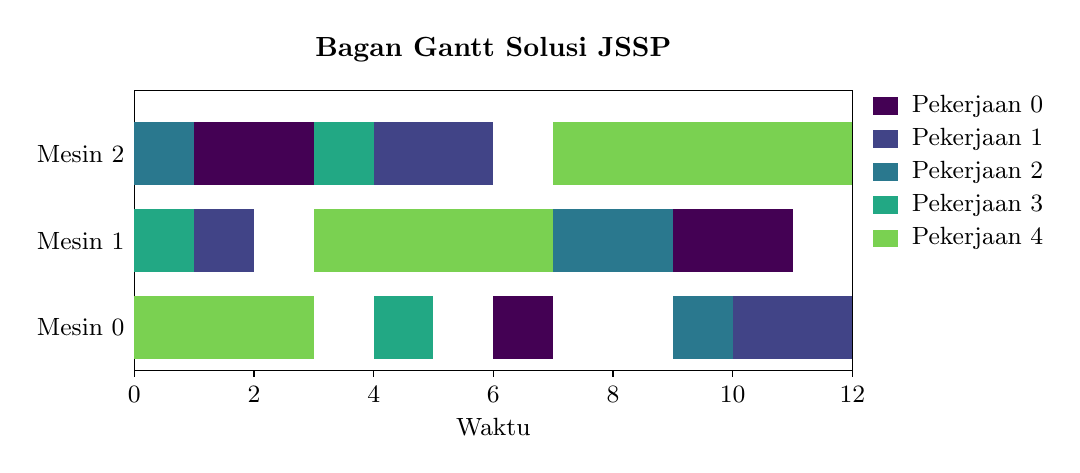
\begin{tikzpicture}[x=0.76cm,y=1.00cm,font=\small]
  \definecolor{jobzero}{HTML}{440154}
  \definecolor{jobone}{HTML}{414487}
  \definecolor{jobtwo}{HTML}{2A788E}
  \definecolor{jobthree}{HTML}{22A884}
  \definecolor{jobfour}{HTML}{7AD151}

  \node[font=\normalsize\bfseries] at (6,4.08) {Bagan Gantt Solusi JSSP};
  \draw (0,0) rectangle (12,3.55);
  \foreach \x in {0,2,...,12} {
    \draw (\x,0) -- ++(0,-0.08);
    \node[below] at (\x,-0.08) {\x};
  }
  \node[below,font=\small] at (6,-0.48) {Waktu};
  \node[left,font=\small] at (0,0.55) {Mesin 0};
  \node[left,font=\small] at (0,1.65) {Mesin 1};
  \node[left,font=\small] at (0,2.75) {Mesin 2};

  % Mesin 0
  \fill[jobfour] (0,0.15) rectangle (3,0.95);
  \fill[jobthree] (4,0.15) rectangle (5,0.95);
  \fill[jobzero] (6,0.15) rectangle (7,0.95);
  \fill[jobtwo] (9,0.15) rectangle (10,0.95);
  \fill[jobone] (10,0.15) rectangle (12,0.95);
  % Mesin 1
  \fill[jobthree] (0,1.25) rectangle (1,2.05);
  \fill[jobone] (1,1.25) rectangle (2,2.05);
  \fill[jobfour] (3,1.25) rectangle (7,2.05);
  \fill[jobtwo] (7,1.25) rectangle (9,2.05);
  \fill[jobzero] (9,1.25) rectangle (11,2.05);
  % Mesin 2
  \fill[jobtwo] (0,2.35) rectangle (1,3.15);
  \fill[jobzero] (1,2.35) rectangle (3,3.15);
  \fill[jobthree] (3,2.35) rectangle (4,3.15);
  \fill[jobone] (4,2.35) rectangle (6,3.15);
  \fill[jobfour] (7,2.35) rectangle (12,3.15);

  \begin{scope}[shift={(12.35,3.25)}]
    \fill[jobzero] (0,0) rectangle (0.42,0.22);
    \node[right] at (0.48,0.11) {Pekerjaan 0};
    \fill[jobone] (0,-0.42) rectangle (0.42,-0.20);
    \node[right] at (0.48,-0.31) {Pekerjaan 1};
    \fill[jobtwo] (0,-0.84) rectangle (0.42,-0.62);
    \node[right] at (0.48,-0.73) {Pekerjaan 2};
    \fill[jobthree] (0,-1.26) rectangle (0.42,-1.04);
    \node[right] at (0.48,-1.15) {Pekerjaan 3};
    \fill[jobfour] (0,-1.68) rectangle (0.42,-1.46);
    \node[right] at (0.48,-1.57) {Pekerjaan 4};
  \end{scope}
\end{tikzpicture}
\caption{Solusi penjadwalan job shop yang ditampilkan sebagai bagan Gantt.}\label{fig:jssp}% fig-num-auto
\end{figure}
%\refincludefigurestatic[scale = 1.5]{jssp.png}



\paragraph{Penerapan JSSP}
JSSP memiliki banyak penerapan praktis, termasuk:
\begin{itemize}
  \item Manufaktur: Menjadwalkan tugas dalam lini produksi untuk mengoptimalkan keluaran.
  \item Ilmu Komputer: Mengalokasikan tugas ke prosesor dalam lingkungan komputasi paralel.
  \item Layanan Kesehatan: Menjadwalkan pembedahan dan perawatan lain di rumah sakit.
  \item Transportasi: Mengoptimalkan tugas pemeliharaan kendaraan atau pesawat di fasilitas pemeliharaan.
\end{itemize}


\subsection{Model Matematis}

Sekarang kita membangun program bilangan bulat campuran dari unsur-unsur di atas.
Formulasi \emph{disjungtif} ini bersifat klasik dan dikembangkan oleh Manne\footnote{A.~S.~Manne, ``On the Job-Shop Scheduling Problem,'' \emph{Operations Research} 8(2):219--223, 1960.}.

\modelhead{Himpunan}
\begin{itemize}
  \item $J = \{1, \ldots, n\}$, pekerjaan.
  \item $I = \{1, \ldots, m\}$, mesin.
\end{itemize}
\modelhead{Parameter}
\begin{itemize}
  \item $o_r^j$, mesin yang menampung operasi ke-$r$ dari pekerjaan $j$; baris $j$ pada matriks $O$ dalam contoh mencantumkan mesin-mesin ini secara berurutan.
  \item $p_{ij}$, waktu pemrosesan pekerjaan $j$ pada mesin $i$.
  \item $M$, konstanta Big-$M$; total waktu pemrosesan $\sum_{i \in I} \sum_{j \in J} p_{ij}$ selalu merupakan pilihan yang sah, sebagaimana dihitung untuk contoh di atas.
\end{itemize}
\modelhead{Variabel}
Keputusan utama adalah waktu mulai kontinu
$$
s_{ij} = \text{ waktu mulai pekerjaan $j$ pada mesin $i$},
$$
beserta variabel $C_{\max}$ untuk makespan.
Waktu mulai saja tidak dapat menyatakan ``salah satu dari dua pekerjaan ini harus menunggu pekerjaan lainnya,'' sehingga untuk setiap mesin $i$ dan setiap pasangan pekerjaan $j < k$ kita menambahkan variabel biner yang mencatat pekerjaan mana yang didahulukan:
$$
z_{ijk} = \begin{cases} 1, & \text{ketika mesin } i \text{ memproses pekerjaan } j \text{ sebelum pekerjaan } k,\\ 0, & \text{ketika pekerjaan } k \text{ mendapat giliran pertama pada mesin } i\text{,} \end{cases}
\qquad i \in I, \ j,k \in J, \ j < k.
$$

\modelhead{Kendala}
\emph{Presedensi dalam suatu pekerjaan.}
Setiap pekerjaan harus mengikuti rutenya: operasi $r$ dari pekerjaan $j$ tidak dapat dimulai sebelum operasi $r-1$ selesai, yaitu,
$$
s_{o^{j}_{r} j} \geq s_{o^{j}_{r-1} j} + p_{o^{j}_{r-1} j} \qquad \forall j \in J, \ r \in \{2, \dots, m\}.
$$

\emph{Satu pekerjaan pada satu waktu per mesin.}
Tetapkan mesin $i$ dan dua pekerjaan $j < k$.
Kelayakan mengharuskan pekerjaan $j$ meninggalkan mesin sebelum pekerjaan $k$ tiba, $s_{ij} + p_{ij} \leq s_{ik}$, atau sebaliknya, $s_{ik} + p_{ik} \leq s_{ij}$.
Ini tepat merupakan keadaan salah satu pada Bagian~\ref{subsec:either-or}, dan penerapan pola tersebut dengan $z_{ijk}$ sebagai variabel pemilih $\delta$ menghasilkan pasangan Big-$M$
$$
\begin{aligned}
s_{ij} + p_{ij} &\leq s_{ik} + M(1 - z_{ijk}) \qquad \forall i \in I, \ j,k \in J, \ j < k,\\
s_{ik} + p_{ik} &\leq s_{ij} + M z_{ijk} \qquad \forall i \in I, \ j,k \in J, \ j < k.
\end{aligned}
$$
Ketika $z_{ijk} = 1$, pertidaksamaan pertama memaksa pekerjaan $j$ mendahului pekerjaan $k$, sedangkan pertidaksamaan kedua dinonaktifkan; ketika $z_{ijk} = 0$, perannya bertukar.

\emph{Makespan.}
Makespan harus berada di atas waktu selesai operasi terakhir setiap pekerjaan:
$$
C_{\max} \geq s_{o^{j}_{m} j} + p_{o^{j}_{m} j} \qquad \forall j \in J.
$$

\modelhead{Model}
\begin{subequations}
\begin{equation}
\begin{array}{rrlr}
\min
               & C_{\max} \\
\st
&            s_{o^{j}_{r}j} &  \geq s_{o^{j}_{r-1}j} +p_{o^{j}_{r-1}j} & \forall j \in {J}, r \in \{2,\dots,m\} \\
             &      s_{ij} + p_{ij}     & \leq s_{ik} + M (1-z_{ijk}) & \forall i \in {I}, j,k \in {J}, j < k \\
              &     s_{ik} + p_{ik}     & \leq s_{ij} + M z_{ijk} & \forall i \in {I}, j,k \in {J}, j < k \\
            &       C_{\max}          & \geq s_{o^{j}_{m}j} + p_{o^{j}_{m}j} & \forall j \in {J} \\
            &      s_{ij}      & \geq 0 & \forall i \in {I}, j \in {J} \\
           &       z_{ijk}     & \in \{0,1\} & \forall i \in {I}, j,k \in {J}, j < k \\
          &        C_{\max} & \geq 0
              \end{array}
              \end{equation}
\end{subequations}
Baris kendala pertama mengikuti rute setiap pekerjaan. Dua baris berikutnya menetapkan urutan pasangan pekerjaan pada mesin yang sama menurut nilai $z_{ijk}$. Baris keempat memastikan bahwa makespan mencakup waktu selesai setiap pekerjaan.
Menyelesaikan model ini untuk contoh empat pekerjaan, tiga mesin di atas memberikan makespan optimal $12$ jam---peningkatan besar dibandingkan $30$ jam yang diperlukan untuk menjalankan pekerjaan satu per satu.
\begin{examplewithallcode}{Penjadwalan Duplo}{}{}{https://github.com/open-optimization/open-optimization-or-examples/blob/master/integer-programming/job-shop-scheduling.ipynb}

Latihan Duplo di kelas diselesaikan dengan Gurobi pada tautan tersebut.

Nilai optimalnya adalah 11.

\begin{center}
% Versi lokal yang dapat diedit menggantikan raster sumber berlabel Inggris.
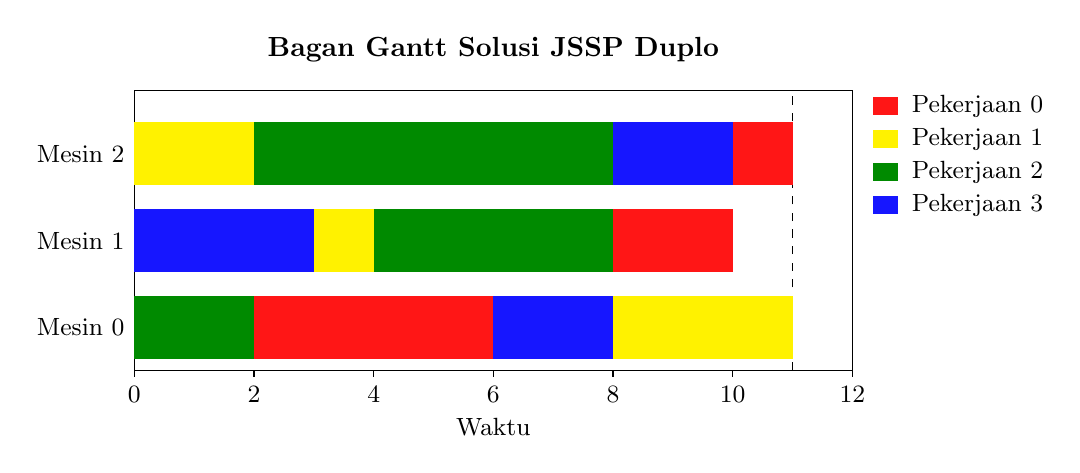
\begin{tikzpicture}[x=0.76cm,y=1.00cm,font=\small]
  \definecolor{duplojobzero}{HTML}{FF1616}
  \definecolor{duplojobone}{HTML}{FFF200}
  \definecolor{duplojobtwo}{HTML}{008A00}
  \definecolor{duplojobthree}{HTML}{1616FF}

  \node[font=\normalsize\bfseries] at (6,4.08) {Bagan Gantt Solusi JSSP Duplo};
  \draw (0,0) rectangle (12,3.55);
  \foreach \x in {0,2,...,12} {
    \draw (\x,0) -- ++(0,-0.08);
    \node[below] at (\x,-0.08) {\x};
  }
  \draw[dashed] (11,0) -- (11,3.55);
  \node[below,font=\small] at (6,-0.48) {Waktu};
  \node[left,font=\small] at (0,0.55) {Mesin 0};
  \node[left,font=\small] at (0,1.65) {Mesin 1};
  \node[left,font=\small] at (0,2.75) {Mesin 2};

  % Mesin 0
  \fill[duplojobtwo] (0,0.15) rectangle (2,0.95);
  \fill[duplojobzero] (2,0.15) rectangle (6,0.95);
  \fill[duplojobthree] (6,0.15) rectangle (8,0.95);
  \fill[duplojobone] (8,0.15) rectangle (11,0.95);
  % Mesin 1
  \fill[duplojobthree] (0,1.25) rectangle (3,2.05);
  \fill[duplojobone] (3,1.25) rectangle (4,2.05);
  \fill[duplojobtwo] (4,1.25) rectangle (8,2.05);
  \fill[duplojobzero] (8,1.25) rectangle (10,2.05);
  % Mesin 2
  \fill[duplojobone] (0,2.35) rectangle (2,3.15);
  \fill[duplojobtwo] (2,2.35) rectangle (8,3.15);
  \fill[duplojobthree] (8,2.35) rectangle (10,3.15);
  \fill[duplojobzero] (10,2.35) rectangle (11,3.15);

  \begin{scope}[shift={(12.35,3.25)}]
    \fill[duplojobzero] (0,0) rectangle (0.42,0.22);
    \node[right] at (0.48,0.11) {Pekerjaan 0};
    \fill[duplojobone] (0,-0.42) rectangle (0.42,-0.20);
    \node[right] at (0.48,-0.31) {Pekerjaan 1};
    \fill[duplojobtwo] (0,-0.84) rectangle (0.42,-0.62);
    \node[right] at (0.48,-0.73) {Pekerjaan 2};
    \fill[duplojobthree] (0,-1.26) rectangle (0.42,-1.04);
    \node[right] at (0.48,-1.15) {Pekerjaan 3};
  \end{scope}
\end{tikzpicture}
\par\captionof{figure}{Bagan Gantt solusi penjadwalan job shop Duplo dengan tiga mesin dan empat pekerjaan berkode warna.}\label{fig:jssp-duplo}% fig-num-auto

%\includegraphicstatic[scale = 0.5]{jssp-duplo}

\includegraphicbook[width=0.24\textwidth, angle=180]{jssp-duplo-actual}\par\captionof{figure}{Foto balok susun Duplo yang diatur sebagai peragaan fisik jadwal job shop.}\label{fig:jssp-duplo-actual}% fig-num-auto

\end{center}
\end{examplewithallcode}

\subsection{Variasi Penjadwalan Job Shop}

Meminimumkan makespan dalam penugasan pekerjaan ke mesin.

Dalam variasi ini, setiap mesin dapat menangani beberapa jenis pekerjaan berbeda. Beberapa mesin dapat menyelesaikan pekerjaan tertentu lebih cepat daripada mesin lain.

Kita ingin meminimumkan waktu penyelesaian semua pekerjaan.

Dalam variasi ini, setiap pekerjaan mengunjungi mesin-mesin yang tercantum secara berurutan: sebagian besar pekerjaan perlu diproses pada dua mesin dalam urutan yang diberikan, sedangkan beberapa hanya memerlukan satu mesin.


%
%
%Misalkan terdapat $n$ pekerjaan dan $m$ mesin.
%
%Misalkan $x_{ij}$ adalah variabel biner yang bernilai 1 jika pekerjaan $i$ ditugaskan ke mesin $j$, dan 0 jika tidak.
%
%Dengan kendala:
%
%Setiap pekerjaan hanya dapat ditugaskan ke satu mesin: $\sum\limits_{j=1}^{m} x_{ij} = 1$ untuk $i=1$ hingga $n$
%
%Setiap mesin hanya dapat memproses satu pekerjaan pada satu waktu: $\sum\limits_{i=1}^{n} x_{ij} \leq 1$ untuk $j=1$ hingga $m$
%
%Waktu mulai suatu pekerjaan didasarkan pada waktu selesai pendahulunya: $y_i \geq y_j + p_j$ untuk $(i,j) \in E$
%
%$y_i \geq 0$ untuk $i=1$ hingga $n$
%
%$x_{ij} \in {0,1}$ untuk $i=1$ hingga $n$ dan $j=1$ hingga $m$
%
%$y_i \in \mathbb{N}$ untuk $i=1$ hingga $n$
%
%Dengan $p_i$ sebagai waktu pemrosesan pekerjaan $i$, dan $E$ sebagai himpunan sisi yang menyatakan kendala presedensi antarpekerjaan.
%
%Model dapat diimplementasikan menggunakan Python dengan pustaka Gurobi sebagai berikut:
%
%\begin{verbatim}
%from gurobipy import *
%
%def job_shop_scheduling(n,m,p,E):
%    # Buat model baru
%    model = Model()
%
%    # Buat variabel
%    x = {}
%    y = {}
%    for i in range(n):
%        y[i] = model.addVar(vtype=GRB.INTEGER, name="y_"+str(i))
%        for j in range(m):
%            x[i,j] = model.addVar(vtype=GRB.BINARY, name="x_"+str(i)+"_"+str(j))
%
%    # Tetapkan fungsi objektif
%    obj = quicksum([y[i]+p[i] for i in range(n)])
%    model.setObjective(obj,GRB.MINIMIZE)
%
%    # Tambahkan kendala
%    for i in range(n):
%        model.addConstr(quicksum([x[i,j] for j in range(m)]) == 1)
%
%    for j in range(m):
%        model.addConstr(quicksum([x[i,j] for i in range(n)]) <= 1)
%
%    for (i,j) in E:
%        model.addConstr(y[i] >= y[j]+p[j])
%
%    for i in range(n):
%        model.addConstr(y[i] >= 0)
%
%    # Optimalkan model
%    model.optimize()
%
%    return
%\end{verbatim}

%Berikut sebuah contoh:
%Berikut sebuah contoh masalah penjadwalan job shop dengan 5 mesin dan 15 pekerjaan:
%
%Mesin 1: Dapat melakukan pekerjaan 1, 2, 3, 4, dan 5
%Mesin 2: Dapat melakukan pekerjaan 6, 7, 8, 9, dan 10
%Mesin 3: Dapat melakukan pekerjaan 11, 12, 13, 14, dan 15
%Mesin 4: Dapat melakukan pekerjaan 1, 6, 11, 2, dan 7
%Mesin 5: Dapat melakukan pekerjaan 3, 8, 13, 4, dan 9
%Pekerjaan:
%
%Pekerjaan 1: Mesin 1 (waktu pemrosesan = 2 jam), Mesin 4 (waktu pemrosesan = 1 jam)
%Pekerjaan 2: Mesin 1 (waktu pemrosesan = 3 jam), Mesin 4 (waktu pemrosesan = 2 jam)
%Pekerjaan 3: Mesin 1 (waktu pemrosesan = 2 jam), Mesin 5 (waktu pemrosesan = 1 jam)
%Pekerjaan 4: Mesin 1 (waktu pemrosesan = 4 jam), Mesin 5 (waktu pemrosesan = 2 jam)
%Pekerjaan 5: Mesin 1 (waktu pemrosesan = 1 jam)
%Pekerjaan 6: Mesin 2 (waktu pemrosesan = 3 jam), Mesin 4 (waktu pemrosesan = 2 jam)
%Pekerjaan 7: Mesin 2 (waktu pemrosesan = 2 jam), Mesin 4 (waktu pemrosesan = 1 jam)
%Pekerjaan 8: Mesin 2 (waktu pemrosesan = 4 jam), Mesin 5 (waktu pemrosesan = 2 jam)
%Pekerjaan 9: Mesin 2 (waktu pemrosesan = 1 jam), Mesin 5 (waktu pemrosesan = 1 jam)
%Pekerjaan 10: Mesin 2 (waktu pemrosesan = 2 jam)
%Pekerjaan 11: Mesin 3 (waktu pemrosesan = 3 jam), Mesin 4 (waktu pemrosesan = 2 jam)
%Pekerjaan 12: Mesin 3 (waktu pemrosesan = 2 jam), Mesin 4 (waktu pemrosesan = 1 jam)
%Pekerjaan 13: Mesin 3 (waktu pemrosesan = 4 jam), Mesin 5 (waktu pemrosesan = 2 jam)
%Pekerjaan 14: Mesin 3 (waktu pemrosesan = 1 jam), Mesin 5 (waktu pemrosesan = 1 jam)
%Pekerjaan 15: Mesin 3 (waktu pemrosesan = 2 jam)
%Objektif: Minimumkan makespan (yaitu, total waktu yang diperlukan untuk menyelesaikan semua pekerjaan)
%
%Kendala:
%
%Setiap pekerjaan hanya dapat dilakukan pada mesin yang ditentukan dalam urutan yang tercantum
%Sebuah mesin hanya dapat mengerjakan satu pekerjaan pada satu waktu
%Tidak ada kendala presedensi antarpekerjaan.
%

\textbf{Mesin:}
\begin{itemize}
    \item Mesin 1: Dapat melakukan pekerjaan 1, 2, 3, 4, dan 5
    \item Mesin 2: Dapat melakukan pekerjaan 6, 7, 8, 9, dan 10
    \item Mesin 3: Dapat melakukan pekerjaan 11, 12, 13, 14, dan 15
    \item Mesin 4: Dapat melakukan pekerjaan 1, 6, 11, 2, dan 7
    \item Mesin 5: Dapat melakukan pekerjaan 3, 8, 13, 4, dan 9
\end{itemize}

\textbf{Pekerjaan:}
\begin{itemize}
    \item Pekerjaan 1: Mesin 1 (waktu pemrosesan = 2 jam), Mesin 4 (waktu pemrosesan = 1 jam)
    \item Pekerjaan 2: Mesin 1 (waktu pemrosesan = 3 jam), Mesin 4 (waktu pemrosesan = 2 jam)
    \item Pekerjaan 3: Mesin 1 (waktu pemrosesan = 2 jam), Mesin 5 (waktu pemrosesan = 1 jam)
    \item Pekerjaan 4: Mesin 1 (waktu pemrosesan = 4 jam), Mesin 5 (waktu pemrosesan = 2 jam)
    \item Pekerjaan 5: Mesin 1 (waktu pemrosesan = 1 jam)
    \item Pekerjaan 6: Mesin 2 (waktu pemrosesan = 3 jam), Mesin 4 (waktu pemrosesan = 2 jam)
    \item Pekerjaan 7: Mesin 2 (waktu pemrosesan = 2 jam), Mesin 4 (waktu pemrosesan = 1 jam)
    \item Pekerjaan 8: Mesin 2 (waktu pemrosesan = 4 jam), Mesin 5 (waktu pemrosesan = 2 jam)
    \item Pekerjaan 9: Mesin 2 (waktu pemrosesan = 1 jam), Mesin 5 (waktu pemrosesan = 1 jam)
    \item Pekerjaan 10: Mesin 2 (waktu pemrosesan = 2 jam)
    \item Pekerjaan 11: Mesin 3 (waktu pemrosesan = 3 jam), Mesin 4 (waktu pemrosesan = 2 jam)
    \item Pekerjaan 12: Mesin 3 (waktu pemrosesan = 2 jam), Mesin 4 (waktu pemrosesan = 1 jam)
    \item Pekerjaan 13: Mesin 3 (waktu pemrosesan = 4 jam), Mesin 5 (waktu pemrosesan = 2 jam)
    \item Pekerjaan 14: Mesin 3 (waktu pemrosesan = 1 jam), Mesin 5 (waktu pemrosesan = 1 jam)
    \item Pekerjaan 15: Mesin 3 (waktu pemrosesan = 2 jam)
\end{itemize}

\textbf{Objektif:} Minimumkan makespan (yaitu, total waktu yang diperlukan untuk menyelesaikan semua pekerjaan)

\modelhead{Kendala}
\begin{itemize}
    \item Setiap pekerjaan hanya dapat dilakukan pada mesin yang ditentukan dalam urutan yang tercantum
    \item Sebuah mesin hanya dapat mengerjakan satu pekerjaan pada satu waktu
    \item Tidak ada kendala presedensi antarpekerjaan.
\end{itemize}
%
%\begin{verbatim}
%job_shop_data = {
%    'machines': {
%        1: {'jobs': [1, 2, 3, 4, 5]},
%        2: {'jobs': [6, 7, 8, 9, 10]},
%        3: {'jobs': [11, 12, 13, 14, 15]},
%        4: {'jobs': [1, 6, 11, 2, 7]},
%        5: {'jobs': [3, 8, 13, 4, 9]}
%    },
%    'jobs': {
%        1: {'machine_times': {1: 2, 4: 1}},
%        2: {'machine_times': {1: 3, 4: 2}},
%        3: {'machine_times': {1: 2, 5: 1}},
%        4: {'machine_times': {1: 4, 5: 2}},
%        5: {'machine_times': {1: 1}},
%        6: {'machine_times': {2: 3, 4: 2}},
%        7: {'machine_times': {2: 2, 4: 1}},
%        8: {'machine_times': {2: 4, 5: 2}},
%        9: {'machine_times': {2: 1, 5: 1}},
%        10: {'machine_times': {2: 2}},
%        11: {'machine_times': {3: 3, 4: 2}},
%        12: {'machine_times': {3: 2, 4: 1}},
%        13: {'machine_times': {3: 4, 5: 2}},
%        14: {'machine_times': {3: 1, 5: 1}},
%        15: {'machine_times': {3: 2}}
%    },
%    'objective': 'minimize_makespan',
%    'constraints': ['job_machine_mapping', 'single_job_single_machine', 'no_job_precedence']
%}
%\end{verbatim}

Pemodelan dan penyelesaiannya kita serahkan sebagai latihan bagi pembaca.

% ============================================================================
% Bagian berikut (QAP, GAP, Materi lain) dibahas dalam Buku 2.
% Buku 1 berfokus pada formulasi pengantar IP.
% ============================================================================

% Bagian QAP dan GAP dipindahkan ke Buku 2
\iffalse  % BEGIN BOOK 2 ONLY CONTENT
\section{Masalah Penugasan Kuadratik (QAP)}
\begin{resource}{}{}
\begin{itemize}
\item \href{https://ieeexplore-ieee-org.ezproxy.lib.vt.edu/stamp/stamp.jsp?tp=&arnumber=7170278}{Kasus terapan masalah penugasan kuadratik pada tata letak departemen rumah sakit}
\item Lihat \href{https://www.semanticscholar.org/paper/Quadratic-Assignment-Problem%3A-A-survey-and-Shawky-Metwally/247b45613d6d3b6961fdad44f9e7fefb70fd3e82}{Masalah Penugasan Kuadratik: Survei dan Penerapan}.
\item \href{https://vtechworks.lib.vt.edu/server/api/core/bitstreams/06b13a4f-d1a9-452c-957f-b0bdd1619c76/content}{Masalah Penugasan Kuadratik dalam Penugasan Gerbang Maskapai untuk meminimumkan jarak berjalan}
\end{itemize}
\end{resource}
Masalah penugasan kuadratik harus memilih penugasan $n$ fasilitas ke $n$ lokasi. Setiap fasilitas mengirimkan sejumlah aliran ke setiap fasilitas lain, dan terdapat jarak antarlokasi yang perlu dipertimbangkan.
Tujuannya adalah meminimumkan hasil kali jarak dan aliran dalam penugasan tersebut.


\begin{example}{Tata Letak Rumah Sakit}{}
Pada suatu hari di rumah sakit, terdapat pasien yang berpindah dari berbagai lokasi di rumah sakit ke berbagai lokasi lainnya. Misalnya, pasien berpindah dari ruang operasi ke ruang pemulihan, atau dari ruang gawat darurat ke ruang operasi, dan sebagainya.

Kita ingin memilih lokasi tempat-tempat tersebut di rumah sakit untuk meminimumkan total jarak yang ditempuh semua pasien.
\end{example}






\begin{general}{Masalah Penugasan Kuadratik}{\npcomplete}
Diberikan aliran $f_{ij}$, hubungan $c_{ij}$, biaya tetap pembangunan $f_i$, permintaan $d_j$, dan kapasitas $u_i$, masalah penentuan lokasi fasilitas berkapasitas adalah

\modelhead{Himpunan}
\begin{itemize}
\item Misalkan $I = \{1,\dots, n\}$ adalah himpunan fasilitas.
\item Misalkan $K = \{1, \dots, n\}$ adalah himpunan lokasi.
\end{itemize}

\modelhead{Parameter}
\begin{itemize}
\item $f_{ij}$ - aliran dari fasilitas $i$ ke fasilitas $j$.
\item $d_{kl}$ - jarak dari lokasi $k$ ke lokasi $l$.
\item $c_{ik}$ - biaya menyiapkan fasilitas $i$ di lokasi $k$.
\end{itemize}

\modelhead{Variabel}
\begin{itemize}
\item Misalkan
\begin{equation*}
x_{ik} = \begin{cases}
1 & \text{jika kita menempatkan fasilitas $i$ di lokasi $k$,}\\
0 & \text{jika tidak.}
\end{cases}
\end{equation*}
\end{itemize}

\modelhead{Model}
\begin{align}
\min \quad & \displaystyle\sum_{i=1}^n\sum_{j=1}^n \sum_{k=1}^n \sum_{l = 1}^n f_{ij}d_{kl}x_{ik}x_{jl} + \sum_{i=1}^n \sum_{k = 1}^n c_{ik} x_{ik}   \tag{biaya total} \\
\st        & \displaystyle\sum_{i=1}^n x_{ik}=1 &&\quad \text{untuk semua } k=1,\dots,n   \tag{tetapkan fasilitas ke lokasi $k$} \\
& \displaystyle \sum_{k=1}^n x_{ik}=1 &&\quad \text{untuk semua } i=1\dots,n   \tag{tetapkan satu lokasi ke fasilitas $i$} \\
& x_{ik}\in\{0,1\} &&\quad \text{untuk semua } i=1,\dots,n, \text{ dan } k = 1, \dots, n   \tag{keputusan biner}
\end{align}
\end{general}

\section{Masalah Penugasan Terampat (GAP)}
\url{https://en.wikipedia.org/wiki/Generalized_assignment_problem}
Dalam \href{applied_mathematics}{matematika terapan},
\textbf{masalah penugasan terampat} maksimum adalah masalah dalam
\href{combinatorial_optimization}{optimisasi kombinatorial}. Masalah ini
merupakan \url{generalization} dari
\href{assignment_problem}{masalah penugasan}, dengan tugas maupun
\href{Agent-based_model}{agen} memiliki ukuran. Selain itu, ukuran setiap
tugas dapat berbeda dari satu agen ke agen lain.

Masalah ini dalam bentuk paling umumnya adalah sebagai berikut: terdapat sejumlah
agen dan sejumlah tugas. Setiap agen dapat ditugaskan untuk melakukan
setiap tugas, yang menimbulkan biaya dan laba tertentu yang dapat berbeda bergantung pada
penugasan agen--tugas. Selain itu, setiap agen memiliki anggaran dan jumlah
biaya tugas yang ditugaskan kepadanya tidak boleh melampaui anggaran tersebut.
Kita perlu mencari penugasan yang membuat semua agen tidak melampaui
anggarannya dan memaksimumkan total laba penugasan.

\hypertarget{in-special-cases}{%
\subsection{Dalam kasus khusus}\label{in-special-cases}}

Dalam kasus khusus ketika semua anggaran agen dan semua biaya tugas
sama dengan 1, masalah ini menyederhana menjadi
\href{assignment_problem}{masalah penugasan}. Ketika biaya dan
laba semua tugas tidak berbeda di antara agen, masalah ini
menyederhana menjadi masalah ransel majemuk. Jika hanya terdapat satu agen,
masalah ini menyederhana menjadi \href{knapsack_problem}{masalah
ransel}.

\hypertarget{explanation-of-definition}{%
\subsection{Penjelasan definisi}\label{explanation-of-definition}}

Dalam uraian berikut, kita memiliki \emph{n} jenis barang, dari \(a_1\) hingga
\(a_n\), dan \emph{m} jenis wadah, dari \(b_1\) hingga \(b_m\). Setiap wadah
\(b_i\) dikaitkan dengan anggaran \(t_i\). Untuk wadah \(b_i\), setiap
barang \(a_j\) memiliki laba \(p_{ij}\) dan bobot \(w_{ij}\). Sebuah solusi
adalah penugasan barang ke wadah. Solusi layak adalah solusi
yang untuk setiap wadah \(b_i\), total bobot barang yang ditugaskan paling
banyak \(t_i\). Laba solusi adalah jumlah laba untuk setiap
penugasan barang--wadah. Tujuannya adalah mencari solusi layak dengan laba
maksimum.

Secara matematis, masalah penugasan terampat dapat dirumuskan sebagai
\href{Integer_programming}{program bilangan bulat}:
\begin{align} \text{maksimumkan } &
\sum_{i=1}^m\sum_{j=1}^n
p_{ij} x_{ij}. \\
\text{dengan kendala } & \sum_{j=1}^n
w_{ij} x_{ij} \le t_i & & i=1,
\ldots, m; \\ &
\sum_{i=1}^m x_{ij} = 1 & & j=1,
\ldots, n; \\ & x_{ij}
\in \{0,1\} & & i=1,
\ldots, m, \quad j=1,
\ldots, n; \end{align}

\section{Materi Lain}

\subsection{Reformulasi Biner Variabel Bilangan Bulat}
Jika variabel bilangan bulat memiliki batas atas dan bawah yang kecil, terkadang ada keuntungan jika variabel tersebut dirumuskan ulang sebagai urutan variabel biner---untuk pemodelan, pemecah, atau keduanya. Meskipun secara teknis ada banyak cara untuk melakukannya, berikut dua cara yang paling umum.

\begin{general}{Reformulasi penuh}{\textcolor{blue}{$u$ variabel biner}}
\label{general:full-reformulation}
Untuk variabel bilangan bulat taknegatif $x$ dengan batas atas $u$, yang dimodelkan sebagai
\begin{equation}
0 \leq x \leq u, \ \ \ \ x \in \Z,
\end{equation}
hal ini dapat dirumuskan ulang dengan $u$ variabel biner $z_1, \dots, z_u$ sebagai
\begin{equation}
\begin{split}
x & = \sum_{i=1}^u i z_i = z_1 + 2 z_2 + \dots + u z_u\\
1 & \geq \sum_{i=1}^u z_i = z_1 + z_2 + \dots + z_u\\
z_i & \in \{0,1\} \ \ \text{ untuk } i=1, \dots, u
\end{split}
\end{equation}
\end{general}
Kita menyebutnya \emph{reformulasi penuh} karena terdapat variabel biner $z_i$ yang terkait dengan setiap nilai $i$ yang dapat diambil oleh $x$. Artinya, jika $z_3 = 1$, kendala kedua memaksa $z_i = 0$ untuk semua $i \neq 3$ (yaitu, $z_3$ adalah satu-satunya variabel biner taknol), dan karena itu menurut kendala pertama, $x = 3$.

\begin{general}{Reformulasi biner}{\textcolor{blue}{$O(\log u)$ variabel biner}}
\label{general:log-reformulation}
Untuk variabel bilangan bulat taknegatif $x$ dengan batas atas $u$, yang dimodelkan sebagai
\begin{equation}
0 \leq x \leq u, \ \ \ \ x \in \Z,
\end{equation}
hal ini dapat dirumuskan ulang dengan $u$ variabel biner $z_1, \dots, z_{\lfloor\log( u )\rfloor}$ sebagai
\begin{equation}
\begin{split}
x & = \sum_{i=0}^{\lfloor\log( u )\rfloor}2^i z_i = z_0 + 2 z_1 +  4 z_2 + 8 z_3 + \dots + 2^{\lfloor\log( u )\rfloor} z_{\lfloor\log( u )\rfloor}\\
z_i & \in \{0,1\} \ \ \text{ untuk } i=1, \dots, \lfloor\log( u )\rfloor
\end{split}
\end{equation}
\end{general}
Kita menyebutnya \emph{reformulasi logaritmik} karena hanya memerlukan variabel biner sebanyak logaritma batas atas $u$. Reformulasi ini terutama lebih baik daripada reformulasi penuh ketika batas atas $u$ merupakan bilangan yang ``lebih besar'', meskipun kita akan membiarkan tetap samar seberapa besar sebuah bilangan harus bernilai agar dapat disebut ``lebih besar''.
\fi  % END BOOK 2 ONLY CONTENT

\section{Latihan}

\exgroup{Pemanasan}

\begin{ex}{Masalah Ransel}{}
\label{ex:knapsack-hiker}
\stars{1} Seorang pendaki mengemas ransel dengan kapasitas berat 15\,kg. Barang yang tersedia adalah:

\begin{center}
\begin{tabular}{c|c|c}
\textbf{Barang} & \textbf{Berat (kg)} & \textbf{Nilai} \\
\hline
Tenda & 5 & 8 \\
Kantong Tidur & 3 & 6 \\
Kompor & 4 & 5 \\
Makanan & 7 & 10 \\
Kamera & 2 & 4 \\
\end{tabular}
\par\captionof{table}{Berat dan nilai barang yang tersedia bagi pendaki.}\label{tab:integerProgrammingFormulations-book1-tab02}% tab-num-auto

\end{center}

\begin{enumerate}
\item Rumuskan program bilangan bulat biner untuk memaksimumkan nilai total barang yang dikemas tanpa melampaui kapasitas berat.
\item Misalkan pendaki juga mengharuskan bahwa jika kompor dikemas, maka makanan juga harus dikemas (Anda tidak dapat memasak tanpa makanan). Tambahkan kendala logis ini ke formulasi Anda.
\end{enumerate}
\exrefs{Contoh~\ref{example:knapsack}, \S\ref{sec:modeling-tricks}}
\end{ex}

\begin{ex}{Ransel Mobil Kurir}{}
\label{ex:knapsack-warmup}
\stars{1} Mobil kurir dapat membawa paling banyak 15\,kg pada perjalanan terakhirnya hari ini. Lima paket menunggu, dengan berat dan imbalan berikut:

\begin{center}
\begin{tabular}{c|c|c|c|c|c}
\textbf{Paket} & 1 & 2 & 3 & 4 & 5 \\
\hline
\textbf{Berat (kg)} & 11 & 3 & 2 & 5 & 4 \\
\textbf{Imbalan (\$)} & 5 & 3 & 3 & 7 & 4 \\
\end{tabular}
\par\captionof{table}{Berat dan imbalan paket untuk mobil kurir.}\label{tab:integerProgrammingFormulations-book1-tab03}% tab-num-auto

\end{center}

\begin{enumerate}
\item Rumuskan masalah ransel biner untuk memilih paket yang akan dimuat.
\item Selesaikan secara manual atau dengan pemecah. Paket mana yang ikut dibawa, dan berapa total imbalannya?
\end{enumerate}
\exrefs{Contoh~\ref{example:knapsack}}
\end{ex}

\begin{ex}{Mencakup Sebuah Kota Kecil}{}
\label{ex:fire-warmup}
\stars{1} Sebuah kota memiliki enam distrik yang tersusun dalam kisi $2 \times 3$:
\begin{center}
\begin{tabular}{|c|c|c|}
\hline
1 & 2 & 3 \\
\hline
4 & 5 & 6 \\
\hline
\end{tabular}
\end{center}
Dua distrik bertetangga jika selnya berbagi satu sisi. Stasiun pemadam kebakaran yang ditempatkan di suatu distrik mencakup distrik tersebut beserta semua tetangganya.
\begin{enumerate}
\item Tuliskan himpunan tetangga $V_i$ untuk setiap distrik $i$.
\item Rumuskan program bilangan bulat penutupan himpunan yang meminimumkan jumlah stasiun pemadam kebakaran sehingga setiap distrik tercakup.
\item Selesaikan contoh tersebut. Berapa banyak stasiun yang diperlukan, dan di mana stasiun-stasiun itu dapat ditempatkan?
\end{enumerate}
\exrefs{Contoh~\ref{example:fire-station}, \ref{general:set-covering}}
\end{ex}

\begin{ex}{Latihan Aktivasi Big-M}{}
\label{ex:bigM-drill}
\stars{1} Sebuah perusahaan tur mengoperasikan tiga wisata dengan jumlah peserta $x_1, x_2, x_3$, dan setiap wisata dapat menampung paling banyak 30 wisatawan ($0 \leq x_i \leq 30$). Misalkan $\delta \in \{0,1\}$ sama dengan $1$ jika perusahaan mempekerjakan pemandu kedua. Kebijakan perusahaan: \emph{jika pemandu kedua tidak dipekerjakan, ketiga wisata secara total hanya dapat menampung paling banyak 40 wisatawan.}
\begin{enumerate}
\item Tuliskan persyaratan jika--maka ini sebagai satu kendala linier menggunakan parameter Big-$M$.
\item Berapa nilai sah terkecil untuk $M$? Berikan pembenaran menggunakan batas-batas $x_i$.
\end{enumerate}
\exrefs{\S\ref{subsec:big-M-activation}, \S\ref{sec:modeling-tricks}}
\end{ex}

\exgroup{Masalah Inti}

\begin{ex}{Menentukan Lokasi Terminal Distribusi}{}
\label{ex:terminals}
\stars{2}
Misalkan sebuah perusahaan yang berbasis di St. John's sedang mempertimbangkan penambahan terminal distribusi di (1) Halifax, (2) Moncton, (3) Montréal, (4) Ottawa, dan (5) Toronto.\\

Biaya pembangunan kelima terminal dalam jutaan dolar adalah 10 di Halifax, 12 di Moncton, 20 di Montréal, 18 di Ottawa, dan 25 di Toronto.
\begin{enumerate}
\item Tidak boleh dibangun lebih dari dua terminal.
\item Jika tidak ada terminal yang dibangun di Halifax, satu terminal harus dibangun di Moncton.
\item Setidaknya satu terminal harus dibangun di Kanada bagian tengah (yaitu di lokasi (3), (4), atau (5)).
\end{enumerate}

Definisikan variabel:
$y_{i}= \begin{cases}1 & \text { jika terminal dibangun di kota } i(i=1, \ldots, 5) \\ 0 & \text { jika tidak}\end{cases}$

Dengan menggunakan variabel ini, tuliskan program bilangan bulat (biner) yang memodelkan masalah penentuan terminal mana yang harus dibangun dengan memenuhi kendala di atas dan meminimumkan biaya.
\exrefs{\S\ref{sec:capital-budgeting}, \S\ref{sec:modeling-tricks}}
\end{ex}

\begin{ex}{Lokasi Gudang}{}
\label{ex:warehouse-cover}
\stars{2} Sebuah perusahaan ritel harus memutuskan lokasi mana dari empat calon lokasi gudang yang akan dibuka. Setiap gudang memiliki biaya tetap pembukaan dan dapat melayani suatu subhimpunan dari lima wilayah pelanggan. Datanya sebagai berikut:

\begin{center}
\begin{tabular}{c|c|l}
\textbf{Gudang} & \textbf{Biaya Tetap (ribuan \$)} & \textbf{Wilayah yang Dilayani} \\
\hline
A & 150 & 1, 2, 3 \\
B & 200 & 2, 3, 4, 5 \\
C & 120 & 1, 4 \\
D & 180 & 3, 4, 5 \\
\end{tabular}
\par\captionof{table}{Biaya tetap pembukaan dan wilayah yang dilayani setiap calon gudang.}\label{tab:integerProgrammingFormulations-book1-tab04}% tab-num-auto

\end{center}

Setiap wilayah pelanggan harus dilayani oleh setidaknya satu gudang yang dibuka.

\begin{enumerate}
\item Definisikan variabel keputusan biner dan rumuskan program bilangan bulat yang meminimumkan total biaya tetap sekaligus memastikan setiap wilayah dilayani.
\item Jenis masalah IP klasik apa yang menyerupai masalah ini?
\end{enumerate}
\exrefs{\ref{general:set-covering}, Contoh~\ref{example:fire-station}}
\end{ex}

\begin{ex}{Penganggaran Modal dengan Kebergantungan}{}
\label{ex:capital-dependencies}
\stars{2} Sebuah perusahaan menyeleksi lima proyek untuk horizon dua tahun. Nilai kini bersih dan pengeluaran kasnya (semuanya dalam \$1000-an) adalah:

\begin{center}
\begin{tabular}{l|c|c|c|c|c}
\textbf{Proyek} & 1 & 2 & 3 & 4 & 5 \\
\hline
\textbf{NPV} & 20 & 40 & 20 & 15 & 30 \\
\textbf{Pengeluaran tahun 1} & 5 & 4 & 3 & 7 & 8 \\
\textbf{Pengeluaran tahun 2} & 1 & 7 & 9 & 4 & 6 \\
\end{tabular}
\par\captionof{table}{Nilai kini bersih dan pengeluaran kas untuk lima calon proyek (dalam \$1000-an).}\label{tab:integerProgrammingFormulations-book1-tab05}% tab-num-auto

\end{center}

Anggaran untuk setiap tahun adalah 20. Selain itu: proyek 3 merupakan perluasan proyek 1 sehingga hanya dapat dijalankan jika proyek 1 dijalankan; dan proyek 2 serta 5 akan melayani pasar yang sama sehingga paling banyak satu di antaranya dapat dipilih.
\begin{enumerate}
\item Rumuskan program bilangan bulat biner yang memaksimumkan total NPV dengan memenuhi kedua anggaran dan kedua kondisi logis.
\item Selesaikan contoh tersebut. Proyek mana yang didanai, dan berapa NPV optimalnya?
\end{enumerate}
\exrefs{\S\ref{sec:capital-budgeting}, \S\ref{sec:modeling-tricks}}
\end{ex}

\begin{ex}{Lokasi Fasilitas: Dua Pusat Distribusi}{}
\label{ex:facility-small}
\stars{2} Sebuah perusahaan dapat membuka pusat distribusi di dua lokasi untuk melayani tiga toko. Biaya pembukaan, kapasitas, biaya pelayanan per unit, dan permintaannya adalah:

\begin{center}
\begin{tabular}{lcc|ccc}
\toprule
 & \(\mathbf{f_i}\) (\$) & \(\mathbf{u_i}\) (unit) & Toko 1 & Toko 2 & Toko 3 \\
\midrule
Pusat 1 & 80 & 40 & \$2 & \$3 & \$1 \\
Pusat 2 & 60 & 25 & \$4 & \$1 & \$2 \\
\midrule
\textbf{Permintaan \(d_j\)} & & & 10 & 12 & 15 \\
\bottomrule
\end{tabular}
\par\captionof{table}{Biaya pembukaan, kapasitas, biaya pelayanan per unit, dan permintaan toko untuk kedua calon pusat.}\label{tab:integerProgrammingFormulations-book1-tab06}% tab-num-auto

\end{center}

\begin{enumerate}
\item Periksa bahwa contoh ini, berbeda dengan contoh distribusi ritel dalam teks, memiliki kapasitas yang cukup agar layak.
\item Rumuskan model lokasi fasilitas berkapasitas untuk data ini.
\item Selesaikan contoh tersebut. Pusat mana yang dibuka, bagaimana permintaan ditetapkan, dan berapa biaya totalnya? Secara khusus, apakah pusat yang lebih murah layak dibuka?
\end{enumerate}
\exrefs{\S\ref{sec:facility-location}}
\end{ex}

\begin{ex}{Mewarnai Graf Lima Simpul}{}
\label{ex:graph-coloring-5}
\stars{2} Pertimbangkan graf dengan simpul $\{A, B, C, D, E\}$ dan sisi
\[
\{A,B\},\ \{B,C\},\ \{C,D\},\ \{D,E\},\ \{E,A\},\ \{A,C\},
\]
yaitu siklus-lima bersama dengan tali busur $\{A,C\}$.
\begin{enumerate}
\item Tuliskan formulasi klasik pemrograman bilangan bulat untuk mewarnai graf ini dengan variabel $x_{ij}$ dan $w_j$.
\item Selesaikan contoh tersebut untuk menemukan bilangan kromatik, dan tunjukkan suatu pewarnaan optimal.
\item Jelaskan bagaimana segitiga $A, B, C$ memberikan batas bawah cepat yang cocok dengan jawaban Anda.
\end{enumerate}
\exrefs{\S\ref{sec:graph-coloring}}
\end{ex}

\begin{ex}{Kendala Salah Satu}{}
\label{ex:either-or-modes}
\stars{2} Sebuah perusahaan memproduksi dua produk, $x_1$ dan $x_2$. Produksi produk~1 memerlukan mesin khusus yang dapat berjalan dalam modus~A atau modus~B, tetapi tidak keduanya secara bersamaan. Kendalanya adalah:
\begin{itemize}
\item Modus A: $2x_1 + x_2 \leq 10$
\item Modus B: $x_1 + 3x_2 \leq 12$
\end{itemize}
Tepat satu dari kedua kendala ini harus berlaku (mesin beroperasi tepat dalam satu modus). Tujuannya adalah memaksimumkan $5x_1 + 4x_2$ dengan $x_1, x_2 \geq 0$.

Perkenalkan variabel biner dan parameter Big-$M$ untuk merumuskan kendala salah satu ini sebagai program bilangan bulat campuran.
\exrefs{\S\ref{subsec:either-or}}
\end{ex}

\begin{ex}{Produksi dengan Biaya Tetap}{}
\label{ex:fixed-charge}
\stars{2} Sebuah pabrik dapat menghasilkan produk dalam kuantitas berapa pun $x \geq 0$, tetapi memulai produksi menimbulkan biaya tetap $\$500$. Biaya produksi variabel adalah $\$8$ per unit, dan setiap unit dijual seharga $\$15$. Pabrik memiliki kapasitas untuk menghasilkan paling banyak 200 unit.

\begin{enumerate}
\item Definisikan variabel biner $y$ yang menunjukkan apakah pabrik memproduksi unit sama sekali. Tuliskan program bilangan bulat campuran yang memaksimumkan laba (pendapatan dikurangi biaya variabel dan biaya tetap).
\item Jelaskan peran kendala yang mengaitkan $x$ dan $y$.
\end{enumerate}
\exrefs{\S\ref{subsec:big-M-activation}}
\end{ex}

\exgroup{Konsep dan Keterkaitan}

\begin{ex}{Mengapa Pembulatan Relaksasi Gagal}{}
\label{ex:lp-rounding}
\stars{2} Kembali ke contoh masalah ransel pada Contoh~\ref{example:knapsack} dan ganti $x_i \in \{0,1\}$ dengan $0 \leq x_i \leq 1$ (relaksasi LP).
\begin{enumerate}
\item Selesaikan relaksasi LP. (Untuk satu kendala ransel, relaksasi dapat diselesaikan secara rakus: urutkan barang berdasarkan nilai per kilogram dan isi tas menurut urutan tersebut dengan mengambil sebagian barang terakhir.) Anda seharusnya memperoleh nilai $52/3 \approx 17.33$ dengan $x_1 = 7/12$ dan semua variabel lainnya sama dengan $1$.
\item Bulatkan variabel pecahan ke atas. Apakah hasilnya layak? Bulatkan ke bawah. Nilai apa yang Anda peroleh, dan bagaimana perbandingannya dengan optimum bilangan bulat sejati sebesar $15$?
\item Dalam kasus ini, pembulatan ke bawah kebetulan memberikan solusi bilangan bulat optimal. Jelaskan mengapa pembulatan secara umum tidak dapat dipercaya. Secara khusus, uraikan dampak pembulatan pada model dengan kendala kesamaan seperti Contoh~\ref{ex:min-coins}, serta pada variabel pilihan biner seperti dalam Latihan~\ref{ex:terminals}, ketika nilai seperti $y_i = 0.5$ tidak memiliki makna.
\end{enumerate}
\exrefs{Contoh~\ref{example:knapsack}, Contoh~\ref{ex:min-coins}, \S\ref{sec:IP-formulations}}
\end{ex}

\begin{ex}{Kapan Big-M Terlalu Besar?}{}
\label{ex:bigM-size}
\stars{2} Dalam Latihan~\ref{ex:either-or-modes}, nilai $M = 10^6$ sepenuhnya sah: program bilangan bulat campuran yang dihasilkan memiliki solusi optimal sama dengan ketika $M = 20$.
\begin{enumerate}
\item Jelaskan dampak $M$ sebesar itu terhadap relaksasi LP: seberapa besar nilai pecahan kecil $\delta$, misalnya $\delta = 10^{-5}$, merelaksasi setiap kendala modus? Mengapa hal ini memperlemah batas yang diperoleh pemecah dari relaksasi?
\item Turunkan konstanta sah yang paling ketat untuk latihan tersebut. Ketika modus B aktif, kendala $x_1 + 3x_2 \leq 12$ membatasi $2x_1 + x_2$; ketika modus A aktif, $2x_1 + x_2 \leq 10$ membatasi $x_1 + 3x_2$. Tunjukkan bahwa $M_1 = 14$ dan $M_2 = 18$ sudah cukup.
\item Sebutkan satu bahaya numerik (titik mengambang) akibat nilai $M$ yang sangat besar sebagaimana disebutkan dalam teks.
\end{enumerate}
\exrefs{Paragraf Memilih Nilai Big-M dalam \S\ref{par:choosing-big-M}, Latihan~\ref{ex:either-or-modes}}
\end{ex}

\begin{ex}{Membaca Model Pertukaran Ginjal}{}
\label{ex:kidney-model}
\stars{2} Pertimbangkan program bilangan bulat pemilihan siklus dalam studi kasus pertukaran ginjal.
\begin{enumerate}
\item Jelaskan dengan bahasa sederhana apa yang diterapkan oleh kendala $\sum_{c \in C:\, i \in c} x_c \leq 1$, dan masalah medis apa yang dapat terjadi jika kendala tersebut dihapus.
\item Fungsi objektif menggunakan koefisien $|c|$. Mengapa $\sum_{c} |c| x_c$ sama dengan jumlah transplantasi yang dilakukan?
\item Himpunan $C$ hanya memuat siklus dengan panjang paling banyak 3. Berikan alasan operasional batas ini, dan uraikan apa yang terjadi pada ukuran $C$ jika batas tersebut dinaikkan.
\item Donor altruistik mendonorkan ginjal tanpa pasien pasangan, sehingga memulai rantai alih-alih siklus. Uraikan cara memperluas himpunan dan variabel model agar mencakup rantai dengan panjang terbatas.
\end{enumerate}
\exrefs{Studi kasus pertukaran ginjal dalam \S\ref{case:kidney-exchange}}
\end{ex}

\exgroup{Masalah Tantangan}

\begin{ex}{Biaya Produksi Linier Sepenggal}{}
\label{ex:pwl-challenge}
\stars{3} Sebuah pabrik dapat menghasilkan hingga 30 ton produk yang dijual seharga \$6 per ton. Biaya produksi bersifat linier sepenggal terhadap kuantitas $x$: 10 ton pertama berbiaya \$5 per ton, 10 ton berikutnya berbiaya \$3 per ton (diskon pembelian masal untuk masukan), dan 10 ton terakhir berbiaya \$8 per ton (lembur).
\begin{enumerate}
\item Tuliskan biaya total $C(x)$ pada titik patah $x = 0, 10, 20, 30$ dan jelaskan mengapa $C$ tidak cembung, sehingga trik LP standar untuk biaya linier sepenggal cembung tidak dapat diterapkan.
\item Rumuskan pemaksimuman laba menggunakan bobot titik patah $\lambda_1, \dots, \lambda_4$ dengan kondisi SOS2, serta tuliskan formulasi variabel biner ekuivalen dari teks.
\item Selesaikan model. Anda seharusnya memperoleh bahwa produksi 20 ton optimal dengan laba \$40. Mengapa pabrik berhenti tepat pada akhir segmen yang mendapat diskon?
\end{enumerate}
\exrefs{\S\ref{subsec:pwl-sos2}, Contoh~\ref{example:pwl}, Contoh~\ref{example:SOS2}}
\end{ex}

\begin{ex}{Dua Pekerjaan, Tiga Mesin}{}
\label{ex:flowshop}
\stars{3} Dua pekerjaan masing-masing harus melalui mesin $M_1 \to M_2 \to M_3$ dalam urutan tersebut. Waktu pemrosesannya adalah:

\begin{center}
\begin{tabular}{l|c|c|c}
 & $M_1$ & $M_2$ & $M_3$ \\
\hline
Pekerjaan 1 & 3 & 2 & 4 \\
Pekerjaan 2 & 2 & 4 & 3 \\
\end{tabular}
\par\captionof{table}{Waktu pemrosesan kedua pekerjaan pada ketiga mesin.}\label{tab:integerProgrammingFormulations-book1-tab07}% tab-num-auto

\end{center}

Setiap mesin hanya dapat memproses satu pekerjaan pada satu waktu, dan pekerjaan tidak dapat diinterupsi.
\begin{enumerate}
\item Perkenalkan variabel waktu mulai $s_{jk}$ untuk pekerjaan $j$ pada mesin $k$ dan tuliskan kendala presedensi dalam setiap pekerjaan.
\item Untuk setiap mesin $k$, perkenalkan variabel biner $\delta_k$ dan tuliskan pasangan kendala Big-$M$ disjungtif yang menyatakan bahwa pekerjaan 1 mendahului pekerjaan 2 pada mesin $k$ atau sebaliknya. Ajukan nilai $M$ yang sah berdasarkan data.
\item Minimumkan makespan dan selesaikan model. Anda seharusnya memperoleh makespan optimal sebesar 12; laporkan pekerjaan mana yang lebih dahulu pada setiap mesin dan jadwal lengkapnya.
\end{enumerate}
\exrefs{\S\ref{sec:job-shop}, \S\ref{subsec:multi-term-disjunction}, \S\ref{subsec:big-M-activation}}
\end{ex}

\subsubsection*{Solusi Terpilih}

\begin{solution}(Latihan~\ref{ex:knapsack-warmup})
Dengan $x_i = 1$ jika paket $i$ dimuat, modelnya adalah
\[
\max\ 5x_1 + 3x_2 + 3x_3 + 7x_4 + 4x_5
\quad \text{dengan kendala} \quad
11x_1 + 3x_2 + 2x_3 + 5x_4 + 4x_5 \leq 15,\ x_i \in \{0,1\}.
\]
Muatan optimal adalah paket $2, 3, 4, 5$ dengan berat $3+2+5+4 = 14 \leq 15$ dan imbalan $3+3+7+4 = \$17$. Paket 1 yang berat tidak pernah menguntungkan: mengambilnya hanya menyisakan ruang 4\,kg, dan hasil terbaik yang dapat dicapai kemudian adalah $5 + 3 = \$8$.
\end{solution}

\begin{solution}(Latihan~\ref{ex:fire-warmup})
Himpunan tetangga (termasuk distrik itu sendiri, seperti dalam contoh stasiun pemadam kebakaran) adalah $V_1 = \{1,2,4\}$, $V_2 = \{1,2,3,5\}$, $V_3 = \{2,3,6\}$, $V_4 = \{1,4,5\}$, $V_5 = \{2,4,5,6\}$, $V_6 = \{3,5,6\}$. Satu stasiun tidak dapat mencakup keenam distrik karena tidak ada himpunan $V_i$ yang memiliki lebih dari empat unsur. Dua stasiun sudah cukup: distrik $2$ dan $5$ mencakup $V_2 \cup V_5 = \{1,\dots,6\}$; begitu pula distrik $3$ dan $4$, serta distrik $1$ dan $6$. Nilai optimalnya adalah $2$, dan ketiga penempatan ini merupakan satu-satunya penempatan optimal.
\end{solution}

\begin{solution}(Latihan~\ref{ex:facility-small})
Kapasitas total adalah $40 + 25 = 65 \geq 37 = 10 + 12 + 15$, sehingga contoh tersebut layak; bahkan pusat 1 saja memiliki kapasitas $40 \geq 37$, sedangkan pusat 2 saja ($25 < 37$) tidak cukup. Dengan menyelesaikan model, optimum membuka pusat 1 saja dan melayani ketiga toko darinya: biaya $80 + 2(10) + 3(12) + 1(15) = 80 + 71 = \$151$. Membuka kedua pusat memerlukan biaya tetap $140$ ditambah biaya pelayanan terbaik $47$, dengan total $\$187$, sehingga pusat yang lebih murah tidak layak dibuka dengan biaya pembukaan \$60.
\end{solution}

\begin{solution}(Latihan~\ref{ex:graph-coloring-5})
Bilangan kromatiknya adalah $3$. Batas bawah: simpul $A$, $B$, $C$ saling bertetangga berpasangan (membentuk segitiga), sehingga memerlukan tiga warna berbeda. Batas atas: pewarnaan $A \to 1$, $B \to 2$, $C \to 3$, $D \to 1$, $E \to 2$ adalah sah, sebagaimana dapat diperiksa sisi demi sisi. Penyelesaian program bilangan bulat mengonfirmasi $\sum_j w_j = 3$.
\end{solution}

\begin{solution}(Latihan~\ref{ex:either-or-modes})
Perkenalkan $\delta \in \{0,1\}$, dengan $\delta = 0$ memilih modus~A dan $\delta = 1$ memilih modus~B. Nilai Big-$M$ yang sah dapat dibaca dari masalah: relaksasikan setiap kendala dengan $M = 20$ (sembarang batas atas ruas kiri pada tingkat produksi yang wajar dapat digunakan). Formulasinya adalah
\[
\begin{aligned}
\max\quad & 5x_1 + 4x_2\\
\text{dengan kendala}\quad & 2x_1 + x_2 \leq 10 + M\delta\\
& x_1 + 3x_2 \leq 12 + M(1-\delta)\\
& x_1, x_2 \geq 0, \quad \delta \in \{0,1\}.
\end{aligned}
\]
Jika $\delta = 0$, kendala modus~A diterapkan dan kendala modus~B direlaksasi; jika $\delta = 1$, perannya bertukar.
\end{solution}

\begin{solution}(Latihan~\ref{ex:fixed-charge})
Misalkan $x \geq 0$ adalah kuantitas produksi dan $y \in \{0,1\}$ menunjukkan apakah produksi dimulai:
\[
\begin{aligned}
\max\quad & 15x - 8x - 500y = 7x - 500y\\
\text{dengan kendala}\quad & x \leq 200\,y\\
& x \geq 0, \quad y \in \{0,1\}.
\end{aligned}
\]
Kendala pengait $x \leq 200y$ memiliki dua peran: jika $y = 0$, kendala tersebut memaksa $x = 0$ (tidak ada produksi tanpa membayar biaya awal), dan jika $y = 1$, kendala tersebut menerapkan batas kapasitas $200$ unit. Karena produksi pada kapasitas menghasilkan $7(200) - 500 = 900 > 0$, solusi optimalnya adalah $y = 1$, $x = 200$.
\end{solution}

\begin{tryit}
\vizlink{branch-bound}{Penjelajah Pohon Branch-and-Bound}: cara pemecah benar-benar menyelesaikan program bilangan bulat dalam bab ini; amati percabangan, pembatasan, dan pemangkasan pada contoh kecil.

\vizlink{concept-quiz}{Kuis Konsep}: dua puluh pertanyaan pemeriksaan mandiri singkat yang mencakup seluruh buku.
\end{tryit}

\section{Literatur dan Sumber Daya}

\begin{resource}



\begin{itemize}
\item Buku pemodelan AIMMS memiliki banyak contoh yang sangat baik. Buku tersebut dapat ditemukan di sini: \href{https://www.aimms.com/english/developers/resources/manuals/optimization-modeling}{AIMMS Modeling Book}.
\item \href{http://web.mit.edu/15.053/www/AMP-Chapter-09.pdf}{Materi Kuliah Terbuka MIT}
\item Untuk berbagai contoh dunia nyata, lihat buku \href{https://link-springer-com.ezproxy.lib.vt.edu/book/10.1007/978-1-4939-1007-6}{
Case Studies in Operations Research
Applications of Optimal Decision Making, disunting oleh Murty, Katta G}.
Atau temukan \href{https://www.springer.com/gp/book/9781493910069}{di sini}.
\item \href{https://github.com/Gurobi/modeling-examples}{Contoh pemodelan GUROBI oleh GUROBI}
\item \href{https://github.com/open-optimization/open-optimization-or-examples/tree/master/integer-programming}{Contoh pemodelan GUROBI oleh Open Optimization yang ditautkan dalam buku ini}
\end{itemize}

Masalah Ransel
\begin{itemize}
\item \href{https://www.youtube.com/watch?v=GteOoMGUOdY}{Video! - Michel Bierlaire (EPFL) mengajarkan masalah ransel}
\end{itemize}

Penutupan Himpunan
\begin{itemize}
\item \href{https://www.youtube.com/watch?v=cjSeHSjPmsk}{Video! - Michel Bierlaire (EPFL) menjelaskan masalah penutupan himpunan}
\item Lihat \href{https://download.aimms.com/aimms/download/manuals/AIMMS3OM_MediaSelection.pdf}{AIMMS - Media Selection} untuk contoh penerapan penutupan himpunan pada pemilihan media.
\end{itemize}

Penentuan Lokasi Fasilitas
\begin{itemize}
\item \href{https://en.wikipedia.org/wiki/Facility_location_problem}{Wikipedia - Masalah Penentuan Lokasi Fasilitas}
\item Lihat \href{https://github.com/Gurobi/modeling-examples/tree/master/facility_location}{Contoh Pemodelan GUROBI - Penentuan Lokasi Fasilitas}.
\end{itemize}


{Contoh lain}
\begin{itemize}
\item \href{https://www.juliaopt.org/notebooks/JuMP-Sudoku.html}{Sudoku}
\item \href{https://download.aimms.com/aimms/download/manuals/AIMMS3OM_EmployeeTraining.pdf}{AIMMS - Pelatihan Karyawan}

\item \href{https://download.aimms.com/aimms/download/manuals/AIMMS3OM_MediaSelection.pdf}{AIMMS - Pemilihan Media}

\item \href{https://download.aimms.com/aimms/download/manuals/AIMMS3OM_Diet.pdf}{AIMMS - Masalah Diet}

\item \href{https://download.aimms.com/aimms/download/manuals/AIMMS3OM_FarmPlanning.pdf}{AIMMS - Masalah Perencanaan Pertanian}

\item \href{https://download.aimms.com/aimms/download/manuals/AIMMS3OM_Pooling.pdf}{AIMMS - Masalah Pooling}

\item \href{https://www.informs.org/Impact}{INFORMS - Dampak}
\item \href{https://www.informs.org/Impact/O.R.-Analytics-Success-Stories/Optimized-school-bus-routing-helps-school-districts-design-better-policies}{INFORMS - Kisah Sukses - Perutean Bus}
\end{itemize}

{Catatan dari buku pemodelan AIMMS.}
\begin{itemize}

\item \href{http://inside.mines.edu/~anewman/MIP_practice120212.pdf}{AIMMS - Panduan praktis untuk menyelesaikan MILP yang sulit}

\item \href{https://download.aimms.com/aimms/download/manuals/AIMMS3OM_LinearProgrammingTricks.pdf}{AIMMS - Trik Pemrograman Linier}


\item \href{https://download.aimms.com/aimms/download/manuals/AIMMS3OM_FormulatingOptimizationModels.pdf}{AIMMS - Merumuskan Model Optimisasi}


\item \href{https://pdfs.semanticscholar.org/b01f/ad44c20c372fdda95cbfb980c0d37302de07.pdf}{AIMMS - Panduan praktis untuk menyelesaikan program linier yang sulit}
\end{itemize}

Trik Pemodelan
\begin{itemize}
\item \href{https://jump.dev/JuMP.jl/stable/tutorials/linear/tips_and_tricks/}{Tip dan trik JuMP}
\item \href{https://docs.mosek.com/modeling-cookbook/mio.html}{Buku Resep Pemodelan Mosek}
\end{itemize}


{Topik Lanjutan}
\begin{itemize}
\item \href{https://or.stackexchange.com/questions/1319/best-model-for-precedence-constraints-within-scheduling-problem}{Kendala Presedensi}
\end{itemize}
\end{resource}

%\end{document}
